%\documentclass[12pt,a4paper,twoside]{book}
% @PETER
\documentclass[12pt,a4paper,twoside,parskip=full]{book}

%include the configuration file for layout
%Have a look in this file it has some useful commands defined
\input{config.tex}

\begin{document}

% @TODO This may be wrong
% Justify Document

%The prelude is everything upto the start of chapter 1
\include{prelude}

%include as many chapters as you have.
%the chapters are in a directory called Chapters
\chapter{Chapter 1 Title}
\label{chapter1}

\section{Starting section}

\newtheorem{w-algorithm}{The W Detection Algorithm is Correct.}

\begin{proof}
After running the BFS twice we obtain two vertices $u$ and $v$ such that:
\begin{equation}
    \label{eq:su_all}
    w(s, u) \ge w(s, t), \forall t \in V(T)
\end{equation}

\begin{equation}
    \label{eq:uv_all}
    w(u, v) \ge w(u, t), \forall t \in V(T)
\end{equation}

Furthermore let $a$ and $b$ be two leaves that define a W Path. Consequently $a$ and $b$ we know that:
$$w(a, b) \ge w(c, d), \forall c, d \in V(T) $$

As $w(u, v) \le w(a, b)$, our end goal here is to bound $w(u, v)$ from bellow in terms of $w(a, b)$. Let also $t$ be the first vertex in the path between $a$ and $b$ that the first BFS starting at $s$ discovers. Clearly $t$ cannot be $a$ or $b$ unless $s$ is equal to $a$ or $b$.

\newpage
This splits into several cases: \linebreak

{\em Case 1. When the path from $a$ to $b$ does not share any vertices with the path from $s$ to $u$.}

{\em Case 1.1. When the path from $u$ to $t$ goes through $s$.}

As $s \rightsquigarrow u$ is a subpath of $t \rightsquigarrow u$ then $w(t, u) \ge w(s, u)$. We also have that $w(s, u) \ge w(s, a)$ by equation \ref{eq:uv_all}. We can therefore conclude that $w(t, u) \ge w(s, a) \ge w(a, t)$ as $s \rightsquigarrow a$ is a subpath of $t \rightsquigarrow a$.


Now via path decomposition we have that:

$$ w(a, b) = w(b, t) + w(t, a) + x  $$
$$ w(u, b) = w(b, t) + w(t, u) + y .$$

Where $x, y \in \{0, 1\}$ depending on whether there is a kink at $t$ for the path from $a$ to $b$ and from $u$ to $b$ respectively. As $w(t, u) \ge w(a, t)$ we can show that:


$$ w(u, b) \ge w(b, t) + w(t, a) + y $$
$$ w(u, b) \ge w(b, t) + w(t, a) + x - x + y $$
$$ w(u, b) \ge w(a, b) - x + y $$
$$ w(u, b) \ge w(a, b) + (y - x) $$

But as $w(u, v) \ge w(u, b)$ (by equation \ref{eq:uv_all}) we obtain that:
$$ w(u, v) \ge w(a, b) + (y - x) $$

Considering all possible values $x$ and $y$ can take, we can see that the minimum value for the right hand side of the equation is at $y = 0$ and $x = 1$. The final conclusion we may draw is that $w(u, v) \ge w(a, b) -1$.



%$a\rightsquigarrow b$

{\em Case 1.2. When the path from $u$ to $t$ does not go through $s$.}

{\em Case 2. When the path from $a$ to $b$ shares at least one vertex with the path from $s$ to $u$.}

\end{proof}

\cite{parikh1980adaptive}

% @TODO Change this
\chapter{Background}
\label{chapter2}

The two key concepts we will introduce in this dissertation are the Contour Tree and Persistent Homology. In order to be able to do this we have to first take a step back and walk the reader through a range of other mathematical disciplines. The preliminaries include Point Set Topology, Differential Topology and Algebraic Topology. We will opt for introducing these fields with a more practical and computational flavour and provide the reader with both the necessary formalism and intuition behind the main definitions and results we will use in the following chapters.

\section{Point Set Topology}

The first branch of Topology we shall encounter is Point Set Topology. It forms the underlying framework on top of which mathematicians build the concepts of continuous spaces and functions. As with many other mathematical disciplines topology is the study of sets that posses mathematical structure. Through point set topology we can define the mathematical structure known as the topology of a set. The topology of a set aims make rigorous the notion of whether two elements of a set are "close" or "near" each other. Elements of a set which are close or near to one another are said to be a part of an open set. We can use the topology of a set to manipulate open sets by combining them to obtain new open sets. In this chapter we will borrow our definitions from one of the standard introductory topology textbooks \cite{intro-topo}.

\begin{defn} Let $X$ be a set and $\tau$ be a set of subsets of $X$. The set $\tau$ is a topology on $X$ when the following holds:  \end{defn}

\begin{itemize}
    \item $X \text{ and } \emptyset \in \tau$.
    \item If $U \text{ and } V \in \tau$ then $U \cap V \in \tau$.
    \item If $\{U_\lambda\}_{\lambda \in \Lambda}$ is a family of subsets of $X$, where $U_\lambda \in \tau$ for all $\lambda \in \Lambda$, then
        $\bigcup_{\lambda \in \Lambda}{U_\lambda} \in \tau$.
\end{itemize}

We will call the elements of $X$ points and the elements of $\tau$ open sets or simply open. An open set is an open neighbourhood of a point when the point is in the open set. We must stress that the topology we endow on a set is by no means unique. For example if $X$ is any set then one topology may be $\{\emptyset, X\}$ and another may consist of all subsets of $X$.

Let us now introduce the topology we are going to use on $\mathbb{R}^n$. It is called the standard topology and it is based on the standard definition of distance between points in Euclidean space. Let $x = (x_1, x_2, ..., x_n)$ be a point in $\mathbb{R}^n$. Then we can define the open ball around $x$ of radius $\epsilon$ as $B_\epsilon(x) = \{y \in \mathbb{R}^n: d(x, y) < \epsilon\}$ where we define the distance function as $d(x, y) = \sqrt{\sum_{i=1}^n{(x_i - y_i)^2}}$. The standard topology on $\mathbb{R}^n$ consists of the open balls around all points of all possible radii and their finite intersections and arbitrary unions.

% But how is it possible to update this? How fast is it? * What do you mean by this? *

The next thing we would like to do is to define a special class of functions that preserve the properties of topological spaces. Those are continuous functions.

\begin{defn} A function $f : X \to Y$ is said to be continuous when the preimage of an open set in $Y$ is an open set in $X$. \end{defn}

In formal notation if $U \in Y$ is open in $Y$ then $f^{-1}(U)$ is open in $X$. This definition captures the intuitive understanding we have of continuity from calculus - if we "slightly adjust" the output of a function in $Y$ then there should be only a "slight change" in input in $X$. The "slight change" is formalised by considering all points in a single open set, as we can think of them as being "near".

% @TODO Add quote
If $f$ is a bijection and $f^{-1}$ is also continuous we will call $f$ a homeomorphism. Homeomorphisms play a special role in topology. Two topological spaces are homeomorphic when there exists a homeomorphism between then. As continuous functions preserve open sets it follows that the two spaces are topologically identical. This is the reason why topologists are mostly interested in classifying and analysing spaces up to homeomorphism. We will call a property of a space that is preserved under homeomorphisms a topological invariant.

%Homeomorphism is the appropriate equivalence relation for topological spaces [].

Now let us introduce our first topological invariant - path connectedness. It captures the idea of a topological space where there is a path between any two of its points.

\begin{defn} Let $X$ be a topological space and let $x, y \in X$ be any two points. A path between $x$ and $y$ in $X$ is a continuous function $f: [0, 1] \to X$ such that $f(0) = x$ and $f(1) = y$.  \end{defn}

% @TODO Add this
Using this definition we can define a path-connected topological space as follows.

\begin{defn} A topological space $X$ is said to be path-connected if there exists a path between any two points $x, y \in X$  \end{defn}

This deceptively simple looking definition actually describes one of the methodologies for analysing topological spaces. Through defining auxiliary some auxiliary structure. In the case of path-connectedness we have employed a two parameter family of utility functions to "measure" a global property of the topological space - whether it is path connected or not. The two parameter family is the collection of all paths between all pairs of points.

An important property of path-connectedness is that the continuous image of a path-connected topological space is also path-connected. Properties like this are crucial in the task of differentiating between topological spaces. If for example one space is path-connected and another one is not there there cannot exists a homeomorphism between them. Consequently they are not homeomorphic and therefore topologically different.

We will now introdue two different way in which you can obtain new topologies from already known topologies. The first way is through the subspace topology. A subspace of a topological space $X$ is any subset of points in $X$.

\begin{defn} Let $A \subseteq X$ be a suspace of $X$. The we define the open sets for a topology on $A$ as the intersection of the open sets in $X$ with $A$. \end{defn}

This means that a set $U \subseteq A$ is open in $A$ exactly when $U = U' \cap A$ where $U'$ is open in $X$. This powerful result allows us to obtain a topology through taking all possible intersections of the open sets in $X$ with $A$. For example let $X = \mathbb{R}$ and $A = [0, 1]$. The set $[0, 1/2) = (-1/2, 1/2) \cap [0, 1]$ is open in $A$ because $(-1/2, 1/2)$ is open in $X$, however the resulting set of the intersection
$[0, 1/2)$ is not open in $X$ (only in $A$).

The second way of obtaining new topologies is via the quotient topology. To understand it we must first define a quotient space. An equivalence relation $\sim$ defined on a topological space $X$ partitions all points in $X$ into equivalence classes. The equivalence class of a point $x \in X$ is the set $[x] = \{y \in X: x \sim y\}$. The set of all equivalence classes is called the quotient of $X$ by $\sim$ and denoted as $X / \sim$. Let also $\pi: X \to X/ \sim$ be the map that takes a point $x$ of $X$ to its equivalence class in $X / \sim$.

\begin{defn} Let $X$ be a topological space and $\sim$ be an equivalen relation defined on $X$. The quotient topology of $X / \sim$ is formed by the sets $U \subseteq X / \sim$ such that $\pi^{-1}(U)$ is open in $X$. \end{defn}

By this definition the function $\pi$ is continuous. We can use this fact to infer that if a topological space $X$ is path-connected then $X / \sim$ is path connected for any equivalence relation $\sim$ because there exists a continuous function $\pi : X \to X / \sim$. An important example is when we take quotients of subsets of topological spaces. Let $A \subseteq X$ and let we can define an equivalence relation as $x \sim y$ whenever both $x, y \in A$. We will call the resulting quotient space $X / A$. The geometrical interpretation of $X / A$ is that all points in $A$ are contracted to a single point and all points in $X$ are left unchanged. As a direct example of this consider the closed disk $D = \{x^2 + y^2 \le 1\}$ and its subset the circle $S^1 = \{x^2 + y^2 = 1\}$.
Then $D / S^1$ is homeomorphic to the three dimensional sphere $S^2 = \{x^2 + y^2 + z^2 = 1\}$. To see why this is true imagine embedding $D$ in the $xy$ plane of a three dimensional space. Now imagine contracting all points along $S^1$ to a single point above the $xy$ plane. The resulting object resembles $S^2$ but with a cusp.

Now we will present our final definition. That of a topological manifold - a mathematical generalisation of a surface.

\begin{defn} A $d-manifold$ is topological space where every point has an open neighbourhood that is homeomorphic to $\mathbb{R}^d$.  \end{defn}

% @TODO Redo last sentence.
Examples of 0-dimensional manifolds are points. Examples of one dimensional manifolds are lines, circles, graphs and curves. Examples for 2-dimensional manifolds are the surfaces we are familiar with from geometry such as the sphere, the torus and so on. In this dissertation we will exclusively be using manifold of dimension up to two. * This is because we are most interested in the visualisation aspect of computational topology and hence would like to limit ourselves to modelling spacial phenomena of up to three dimensions. *

% *Manifolds are the playground where topology meets geometry.*

It is often hard to analyse the topology of a space by just considering its open sets. * In practice it is even computationally infeasible due to the shear number of ways we can combine open sets. * This is why in the following two chapters we will employ additional tools from other fields of mathematics to aid in our analysis of the topology of a space. Two such tools are differentiable function over differentiable spaces and combinatorial approximations of topological spaces.


%Contractable Space.

%Path Connected Space.

%Homotopy.

%All of the low level stuff.

%Manifolds.

%Submanifold.

%Genus of a manifold.


%It is often hard to analyse a space just using it's topology.

%This is why we will use additional tools to investigate the topology of a space.

%Two such tools are differentiable function and decomposition into a simplical complex.

\section{Differential Topology}

Differential topology is the study of differentiable functions defined on differentiable manifolds. One of the leading fields of differential topology is that of Morse Theory \cite{morse-theory-book, morse-theory-book-milnor}. Morse theory is the study of the relation between spaces and functions defined on them. One of the main goals is to determine the shape of a shape by analysing the class of functions that can be defined on it. For example using methods from differential topology we can show that the real line and the circle are different topologically. * See Appendix for example.*

One way we can study smooth manifolds via differentiable functions is by analysing the critical points of the functions. This however is an enormous task in its own right. This is why we will restrict ourself to a special class of differentiable functions called Morse functions.

\begin{defn} A function $f: M \to \mathbb{R}^n$ is a Morse Function if $f$ is smooth and at critical points the Hessian (matrix of second partial derivatives) is full rank.   \end{defn}

For practical considerations we will restrict our attention even further and consider Morse functions whose codomain is $\mathbb{R}$. One way we can use a Morse function defined on a manifold is to decompose the manifold into a family of nested subsets. We can then analyse the subsets to obtain some global topological information. Examples of such familiest of subsets are level sets, sublevel sets and super level sets.

\begin{defn} A level set at a value $h$ of a Morse function $f: M \to \mathbb{R}$ is the set $f^{-1}(\{h\}) = \{x \in M: f(x) = h \}$   \end{defn}

Sublevel sets are defined in terms of the preimage of $f$ of intervals of the form $[-\infty, a]$. The sublevel set at $a$ is defined as $f^{-1}([-\infty, a]) = \{x \in M: f(x) \in [-\infty, a] \}$. Superlevel sets are defined analogously in terms of intervals of the form $[a, \infty]$.
% @TODO Include this somewhere else?
% We will call the path-connected components of a level set contours.

% @TODO Explain Critical Points and Critical Value.

Morse functions ensures the following properties which we will make use of in the future:

\begin{itemize}
    \item None of the critical points of a Morse function are degenerate.
    \item Changes in the topology of (sub/super)level sets only happen at critical values. We will call those points critical points.
    \item A Morse function defined on a closed surface has a finite number of critical points.
\end{itemize}

As we saw Morse functions allow us to decompose a manifold into its level sets. We can explore how the connectivity of the level sets changes as we vary the parameter using the abstraction of Reeb Graph.

\subsection{Reeb Graph}

% @TODO Define the quotient topology. Also I'm not sure if you definition of reeb graph is correct!


The Reeb Graph is a tool that encapsulates the evolution of the topology of level sets of a continuous function. When the function is Morse, an edge in the Reeb Graph corresponds to a sequence of contours in the level sets whose topology does not change. The vertices correspond to critical points where the topology of those components does changes. Example of a topological change is when connected components in the level sets appear or dissapear or when two connected components split or merge. * Morse theory ensures that critical points occur at distinct values of the parameter and are isolated. This removes any ambiguities that may arise in the construction of the graph. Furthermore that fact that their number is finite on a close surface and the fact that they only happen at critical values make this computation tractable. *

\begin{defn}
Given a topological space $X$ and a continuous function $f: X \to \mathbb{R}$ we can define an equivalence relation $\sim$ such that two points $x, y$ in $X$ are equivalent when there exists a path between them in a level set $f^{-1}(\{h\})$ for some $h \in \mathbb{R}$. The Reeb Graph is the quotient space $X \big/ \sim$ together with the quotient topology.
\end{defn}

Intuitively we can think of the Reeb Graph of the space where connected components of $X$ are contracted to a single point. We can turn the resulting topological graph into a combinatorial structures by recording all the vertices and edges between them.

*SHOW LOTS OF PICTURES*

The reason we have define reeb graphs is because a contour tree is a special case of the reeb graph. We will come back to this in the begining of the next chapter. Before we move on we must take a look at certain tools from Algebraic Topology that allows us to translate the continuous mathematical results we have obtained so far into the realm of finite combinatorial structures that would allow us to perform actual computation.

\section{Algebraic Topology}

% @TODO Incorrect English in last sentece
Algebraic Topology is a branch of topology that uses tools from the field of abstract algebra to study topological spaces. The primary goal is to derive algebraic structures such as groups, rings and vector spaces from topological spaces that remain invariant under continuous mappings. Modern Algebraic Topology has its roots in combinatorially defined topological spaces \cite{comb-alg-topo}. Unlike Point Set Topology and Differential Topology this allows us to obtain exact algorithm for computing the algebraic invariant we are interested in. To make matters clearer firstly we will introduce one of the most basic combinatorial topological space - Simplicial Comlexes and then we will introduce one of the earliest discovered algebraic invariants - the Euler Characteristic. We will continue our discussion on Algebraic Topology in Chapter Five where we will see how the concept of the Euler Characteristic can be generalised to the one a field of Algebraic Topology called Homology.

\subsection{Simplicial Complexes}

Simplical Complexes are the one of the first combinatorially flavoured topological spaces one encounters in Algebraic Topology. A simplicial complex is a set that consists of points, line segments, triangles and their higher dimensional analogues all "glued together" in a single structure. In order to understand simplicial complexes we must first understand what their basic building blocks are \cite{comp-topo}.

\begin{defn} Let $\{v_0, ..., v_k\}$ be points in $\mathbb{R}^d$. The convex combination of the points is the sum $\sum_{i=0}^k{\lambda_ix_i}$ where $\lambda_i \ge 0$ and $\sum_{i=0}^n{\lambda_i} = 1$.  \end{defn}

If we decide to take the subset of $\mathbb{R}^d$ covered by all possible convex combination we obtain the convex hull of the points.

\begin{defn} Let $\{v_0, ..., v_k\}$ be points in $\mathbb{R}^{k+1}$. We will call the convex combination of those points the $k-simplex$ defined by the points.  \end{defn}

* Show Examples *

\begin{figure}[h]%
    \centering
    \subfloat[Vertex]{{
\includegraphics[scale=0.025]{./images/simplex/vertex.eps}}}%
    \subfloat[Edge]{{
\includegraphics[scale=0.025]{./images/simplex/edge.eps}}}%
    \subfloat[Triangle]{{
\includegraphics[scale=0.025]{./images/simplex/triangle.eps}}}%
    \subfloat[Tetrahedron]{{
\includegraphics[scale=0.025]{./images/simplex/tet.eps}}}%

    \caption{The simplices of dimension $0, 1, 2$ and $3$.}%
    \label{fig:example}%
\end{figure}

In the definition above the number $k$ is also called the dimension of the simplex. * Analogous to how we mentioned that we will only make use of low dimensional manifolds, here we will only be considering simplices of dimension up to three.*  We will call the simplices of dimension $0, 1, 2 \text{ and } 3$ vertices, edges, triangles and tetrahedron respectively.

A face of a simplex is the convex hull of a non-empty subsets of its points. *Thus the points that define the simplex are its vertices.* To obtain a simplical complex all we have to do is take the union of a number of simplices in the same *ambient dimension* and glue them along common faces without allowing self-intersection. More formally:

\begin{defn} A simplical complex $K$ is a finite collection of simplices such that if $\tau$ is a simplex $K$ then all faces of $\tau$ must be simplicies in $K$. Furthermore the intersection of two simplicies in $K$ is either empty or a common face of both.  \end{defn}


\begin{figure}[h]%
    \centering
    
\includegraphics[center, scale=0.03 ]{./images/simplex/complex.eps}
    \caption{A simplicial comlex}%
    \label{fig:case1.1}%
\end{figure}

We shall obtain the topology of a simplex through embedding it in three-dimensional Euclidean space and consider the subspace topology as a subset. Now that we have formalised the concept of a simplical complex let us see what kind of algebraic invariants we can compute from it.


\subsection{Euler Characteristic}

The first topological invariant of algebraic nature we shall encounter is the Euler Characteristic. It is denoted as $\chi$ and it assigns an integer to simplical complexes through a generalisation of counting \cite{elementary-applied-topology}. The concept was originally defined for polyhedra as a alternating sum of the form $|V| - |E| + |F|$, where $V$ is the set of vertices, $E$ the set of edges and $F$ the set of faces. For example this allowed for the classification of the Platonic solids [].

% @TODO Define CW complexes, simplical complexes may not generalise polyhedra
The Euler Characteristic can be generalized to all spaces that can be decomposed into a finite number of cells. Let us first consider simplical complexes *because they generalise polyhedra*. The natural generalisation of the alternating sum is to continue it indefinitely with the number of 3-cells, then 4-cells, etc., as follows

$$ \chi = k_0 - k_1 + k_2 - ... = \sum_{i}{(-1)^i~k_i}, $$

where all $k_i$ is the number of $i$ dimensional simplicies and $k_i = 0$ for $i$ bigger than some $n \in \mathbb{Z}^+$ and all $k_i$ for $i \le n$ are positive integers.

* Show Examples *

\begin{lem}   The Euler Characteristic is homotopy invariant. \end{lem}

This result allows us to compute the Euler Characteristic of topological spaces which are not simplicial complexes. Let us take for example one of the simplest surfaces - the sphere. We will call any simplicial complex that is homeomorphic to the sphere it's triangulation. The most basic triangulation of the sphere is the tetrahedron. Therefore if we wish to compute the Euler Characteristic of the sphere all we need to do is compute the Euler Characteristic of the tetrahedron. We will use a similar process to compute the contour tree in the next chapter. We will start with an assumption that we have a bounded volume in $\mathbb{R}^2$ and we will triangulate it to enable computation of a topolthe conture tree.

%This results allows to compute in practice $\chi$ of manifolds by considering any of their finite triangulations. As long as there is a homeomorphism between a manifold and triangulation $\chi$ will not change. We will be well advised to pick the triangulations with the least number of simplices to improve computational efficiency. For example the octahedron is a triangulation of a sphere and therefore the Euler Characteristic of the sphere is zero. For further information on this subject we refer the reader to [].

% @TODO Change this
\chapter{Contour Trees}
\label{chapter3}

% @TODO Add quote reeb graph intro.
The Reeb graph of a scalar field is connected and acyclic \cite{comp-topo}. As such we will call the Reeb graph of a scalar field the contour tree. In this chapter we will assemble the theory we have presented thus far and use it to introduce the state of the art serial and parallel algorithms for contour tree computation. We will begin with a short discussion on how we treat input data and what theoretical simplifying assumptions we are making. Afterwards we will present an overview of contour tree algorithms and then introduce some graph theoretical properties of contour trees. Next we will describe in detail how the serial and parallel contour tree algorithm work. This will lead us to defining the so called w-structures. We will demonstrate why exactly they are a pathological case that causes poor performance in the parallel contour tree algorithm. The final topic of this chapter is contour tree simplification. This is the process of identifying and removing parts of the contour tree that are not topologically significant.

\section{Typical Input Data}

% @TODO Add this back if you have the time.

% Such a process is for example the sampling of temperature from a bounded volume of air [] or the height of points over a geographic region []. The contour tree is shown to be a robust tool primarily used in the visualisation of such natural phenomena [].

Many scientific and medical applications require the sampling of scalar values from a bounded area or volume in two or three dimensional Euclidean space \cite{carr-masters}. The theory we have presented so far is applicable only in the continuous setting but the resolution of any sampling process is finite. If we are to leverage this theory we must assume an underlying continuous function in the whole of the area or volume and not just at the sampled points. To do so we will construct an approximation of this function based on the values we have sampled. This is usually done by constructing a simplicial complex where the data points are the vertices and higher dimensional simplicies are added to completely fill the space between them (see Figure []). We will call the resulting data structure a simplical mesh \cite{carr-masters}.

\begin{figure}[h]%
    \centering
    \subfloat[Input Data]{{\includegraphics[scale=0.06]{./images/w3x3/w3x3-vertices.pdf}}}%
    \qquad \qquad \qquad
    \subfloat[Simplicial Mesh]{{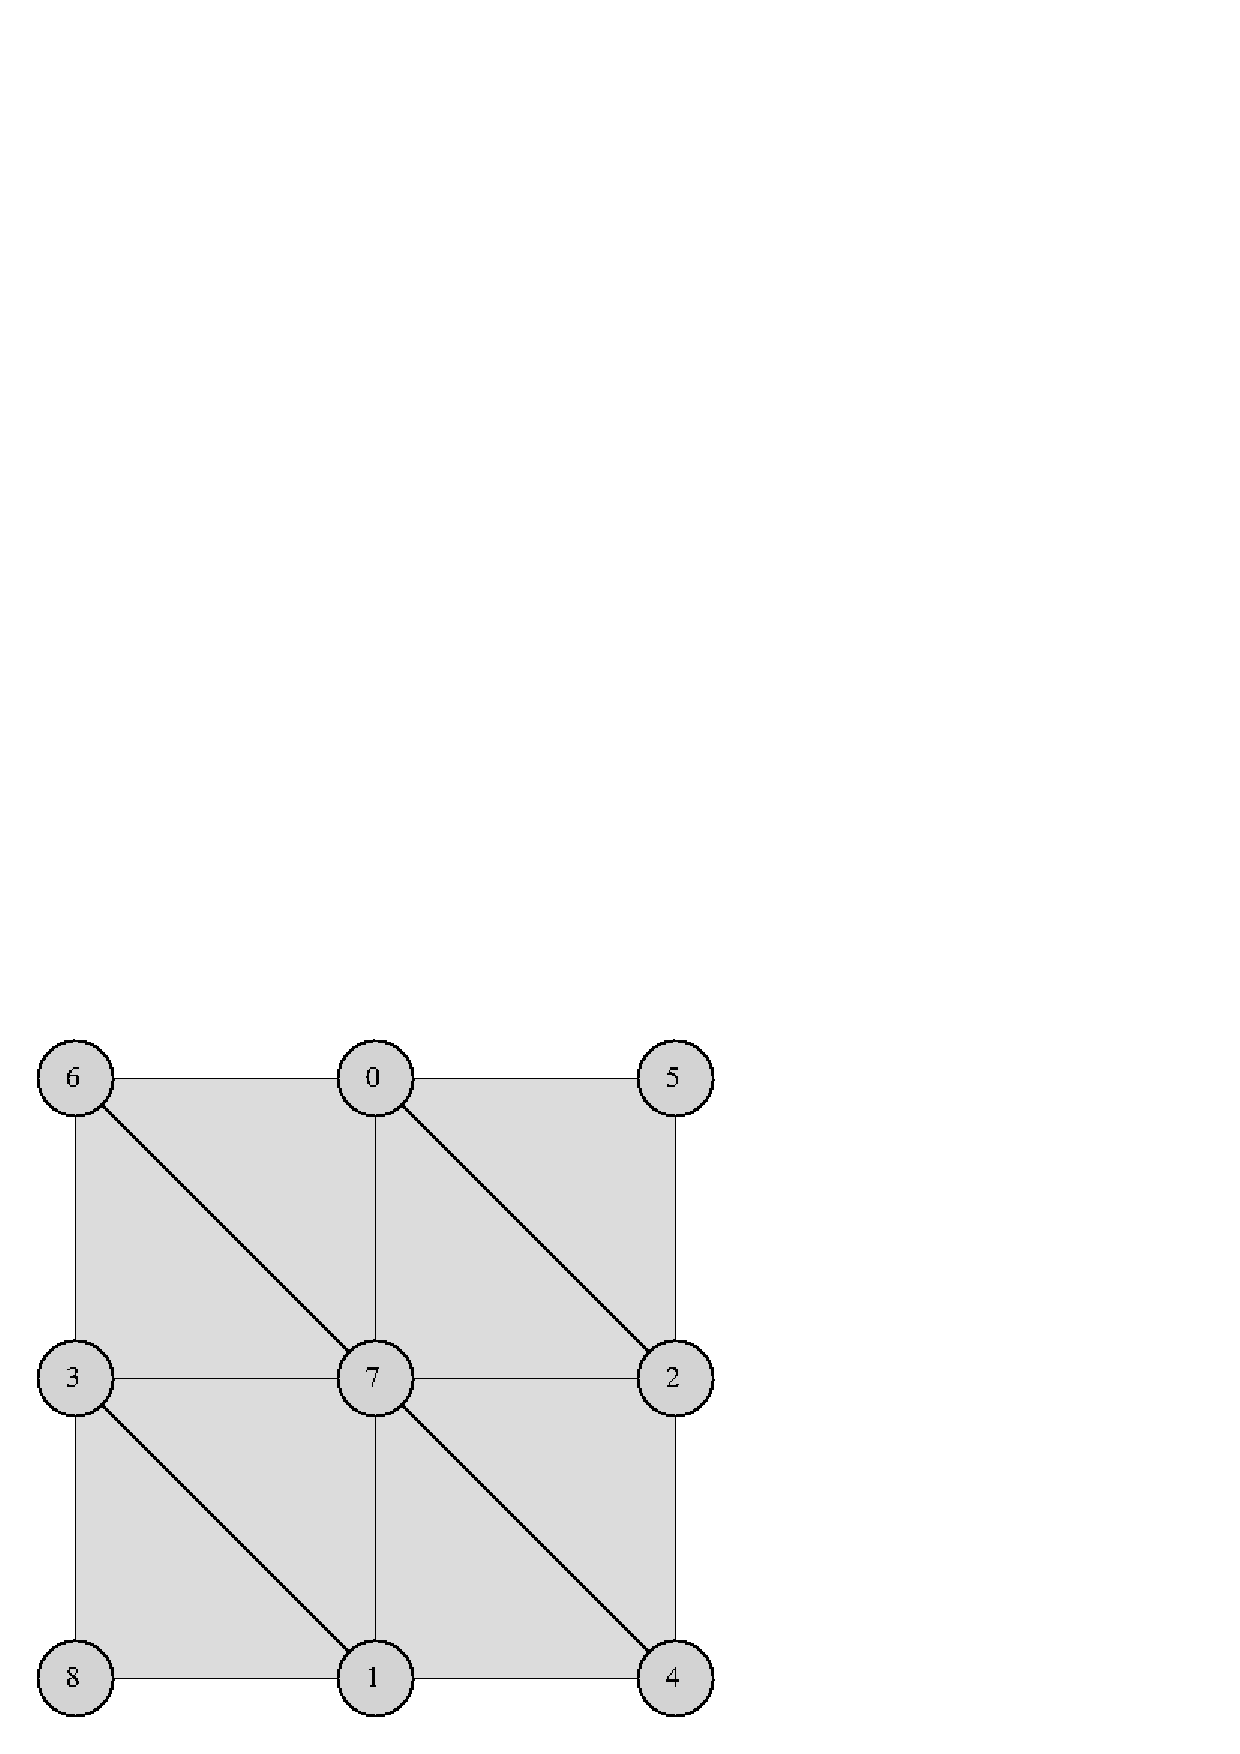
\includegraphics[scale=0.06]{./images/w3x3/w3x3-mesh.pdf}}}%
    \caption{Triangulation of input data to obtain a simplicial mesh.}%
    \label{fig:simplicial-mesh}%
\end{figure}
For simplicity and without loss of generality we will work with two-dimensional domains where the value samples are evenly spaced out in a grid-like fashion (Figure \ref{fig:simplicial-mesh}). The values of the approximation function at the simplicies are obtained via linear interpolation between the verticies of each simplex []. As long as the original values we have sampled are unique it can be shown that the linear interpolation function is a Morse function and that all critical points are the vertices of the mesh \cite{curvature-embeded-polyhedra}.

\section{Contour Tree Computation}


 % @TODO What about higher dimensions and expand parallel stuff?

The first efficient algorithm for constructing contour trees \cite{first-ct-algo} is due to Van Kreveld et al. Its running time is $O(NlogN)$ on two dimensional domains and $O(N^2)$ in higher dimensions where $N$ is the number of triangles in the simplicial mesh. Tarasov and Vyalyi \cite{second-ct-algo} extended this algorithm to work in time $O(NlogN)$ on three dimensional domains. Their approach however involved a complicated procedure for dealing with multi-saddle points. Both algorithms suffer from lack of generality and non-trivial treatment of multi-saddle points. Carr at. al \cite{ct-big-paper} introduced an algorithm with running time $O(nlogn + N\alpha(N))$ where $n$ is the number of vertices in the simplicial mesh and $\alpha$ is the notoriously slow growing inverse Ackerman function. This algorithm works in any number of dimensions and has simple treatment of multi-saddle points.

More recent developments in the field focus on extending the existing algorithms to accomodate the distributed \cite{distributed-ct-algo, distributed-ct-algo-2} and shared memory parallelism paradigms \cite{parallel-peak-pruning, parallel-ct-1}. The focus of this dissertation we will be one of the latest devlopments in a data parallel shared memory algorithm for contour tree computation
\cite{parallel-peak-pruning}. Before introducing how that algorithm operates and one of the issues related to its parallel performance we will first give a more detailed overview of the most established serial algorithm \cite{ct-big-paper} on which the data parallel one is based on. In order to talk about any of the two algorithm we must establish some notation and define height graphs and trees as they are defined in \cite{carr-masters}.

% @TODO Finish this.
% Also define regular points!

\section{Height Trees}

% @TODO Talk about supernodes and superarcs

% @TODO Target application domain.
A height graph is a graph $G = (V, E)$ together with a real valued function $h$ defined on the vertices of $G$. Height graphs are also known in the literature as weighted graphs. We are changing our notation to be more indicative of the fact that the weight function is defined on the vertices and that it corresponds to height in our target application domain. A height tree is a height graph which is a tree. Contour trees are height trees because nodes in the contour tree correspond to nodes in the mesh and can inherit their height (sampled) value. Analogous to the assumption we have made about uniqueness of values we will also assume all vertices in the height trees we consider have unique heights. In other words $h(u) \ne h(v)$ for all $u ,v \in V(G)$ where $u \ne v$. The function $h$ naturally induces a total ordering on the vertices. From now on we will assume the vertices of $G$ are given in ascending order. That is to say, $V(G) = \{v_1, v_2, ... , v_n\}$ where $h(v_1) < h(v_2) < ... < h(v_n)$. This lets us work with the indices of the vertices without having to compare their heights directly. In this notation $h(v_i) < h(v_j)$ when $i < j$.

%@TODO Remove this if you will not use it.

Introducing the height function allows us to talk about ascending and descending paths. A path in a graph is a sequence of vertices $(u_1, u_2, ... , u_k)$ where $u_i \in V(G)$ for $i \in \{1, 2, ..., k\}$ and $u_iu_{i+1} \in E(G)$ for $i \in \{1, 2, ..., k-1\}$. A path in a height graph is ascending whenever $h(u_1) < h(u_2) < ... < h(u_k)$. If we traverse the path in the opposite direction it would be descending. We will simply call these paths monotone whenever we wish to avoid committing to a specific direction of travel.

When working with height graphs it is useful to extend the definition of a degree of a vertex by taking the height function into account.

\begin{defn} Let $G$ be a height graph and $v$ a vertex of $G$. The up degree of $v$ is defined as the number of neighbours of $v$ with higher value. It is denoted as $\delta^+(v) = \big|\{ u \in N(v) : h(u) > h(v) \}\big|$.   \end{defn}

The down degree of a vertex $v$ is defined analogously as $\delta^-(v) = \big|\{ u \in N(v) : h(u) < h(v) \}\big|$. In the context of height trees the definitions of up and down degrees of a vertex allow us distinguish between two types of leafs - lower and upper leafs.
\begin{defn} Let $G$ be a height graph and $v$ a vertex of $G$. If  $\delta^+(v) = 1$ and $\delta^-(v) = 0$ then $v$ is a lower leaf.  \end{defn}

If $\delta^+(v) = 0$ and $\delta^-(v) = 1$ then $v$ is an upper leaf. We will see in the next section how differentiating between the two types of leafs is a crutial part in the computation of the contour tree.

\section{Serial Algorithm}

The contour tree is a tree that consists of []:

\begin{itemize}
    \item Vertices or supernodes that correspond to level sets that contain a critical point.
    \item Edges or superarcs correspond to path-connected regions bounded by two level sets which both contain a critical point. They connect the supernodes those level sets correspond to.
\end{itemize}

% @TODO Think about this contruction and destruction business
The contour tree contains information of four types of events - creation, destruction, joining and splitting of contours. We can derive from the contour tree two other height trees that each contain the information of cretion and joining and destruction and splitting separately. We will call these the join and split trees. The join tree contains information for the contours that are created and joined together and the split tree holds the information for the contours that are destroyed or that split apart. The join tree of a contour tree summarises the evolution of the connectivity of the sublevel sets of the interpolation function and the split tree of the superlevel sets. You can find an example of the join and split trees of Figure \ref{fig:mesh-join-split-contour}.

% The two are symmetric in that the join tree of the function $f$ is isomorphic to the split tree of the negative of the function $-f$.

\begin{figure}[h]%
    \centering
    \subfloat[Simplicial Mesh]{{\includegraphics[scale=0.06]{./images/filtration/asc/x9.pdf}}}%
    \qquad \qquad \qquad
    \subfloat[Contour Tree]{{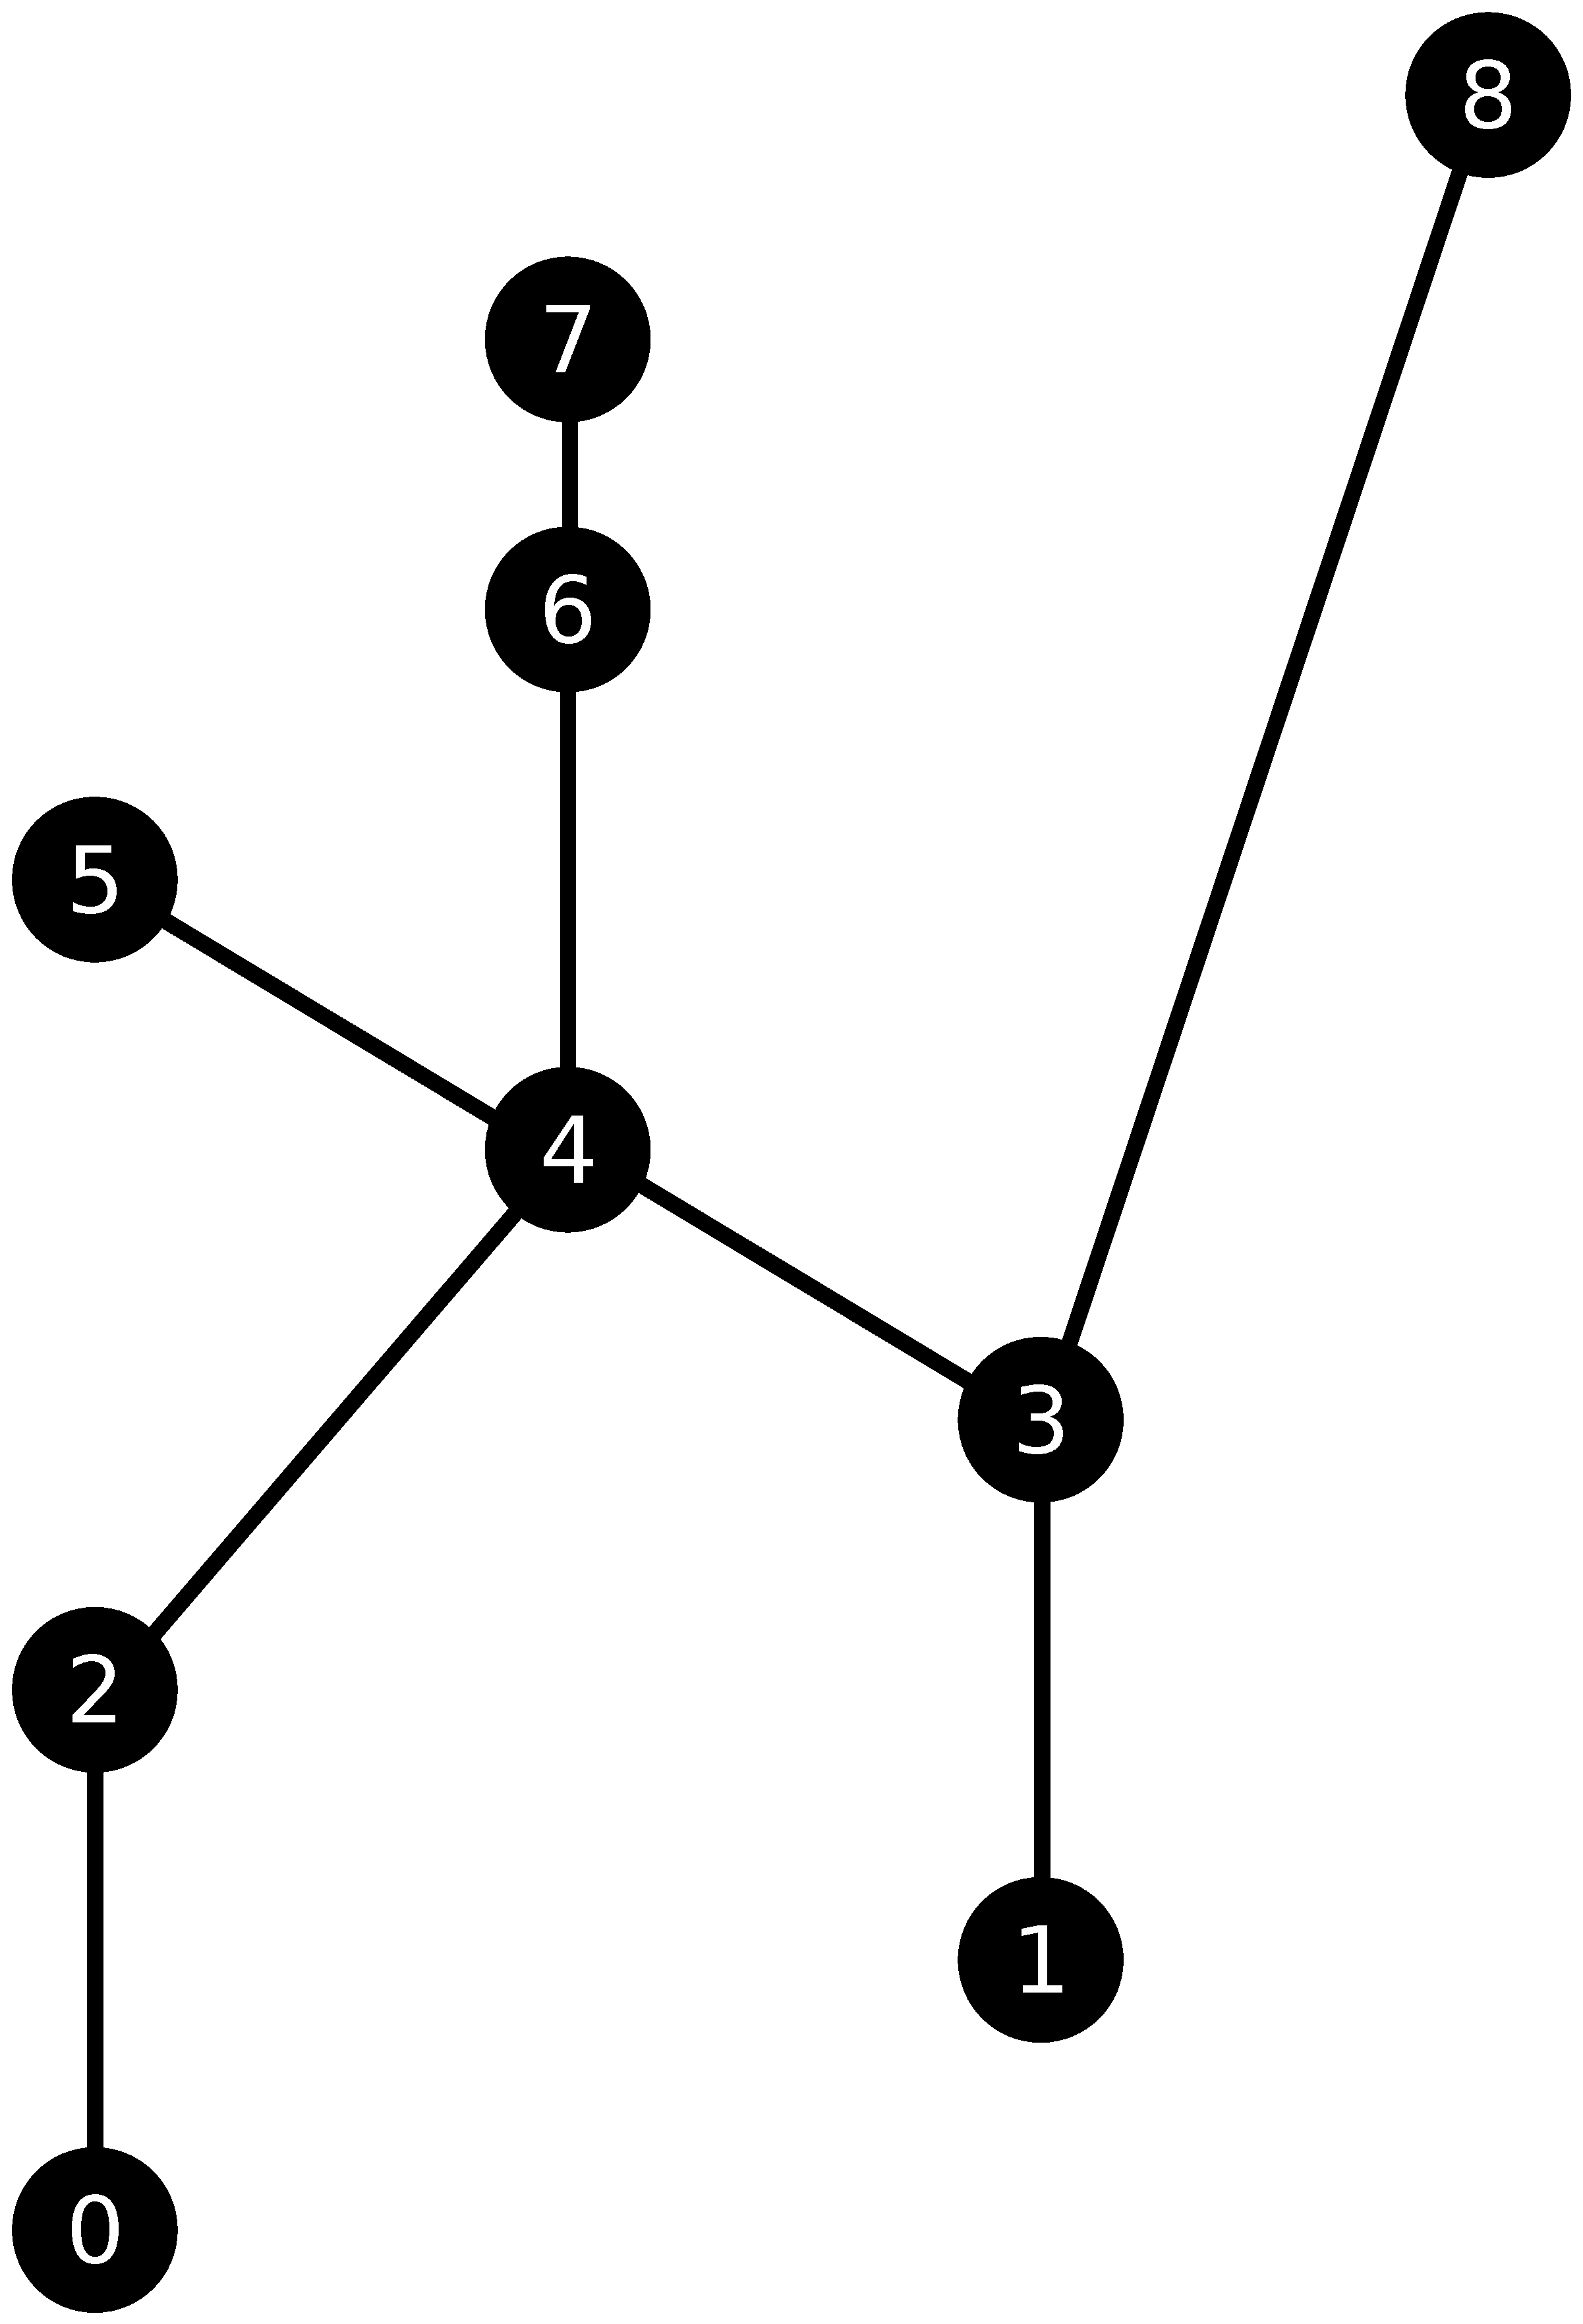
\includegraphics[scale=0.10]{./images/w3x3-contour-tree-new.eps}}}%
    \qquad \qquad \qquad

    \subfloat[Join Tree]{{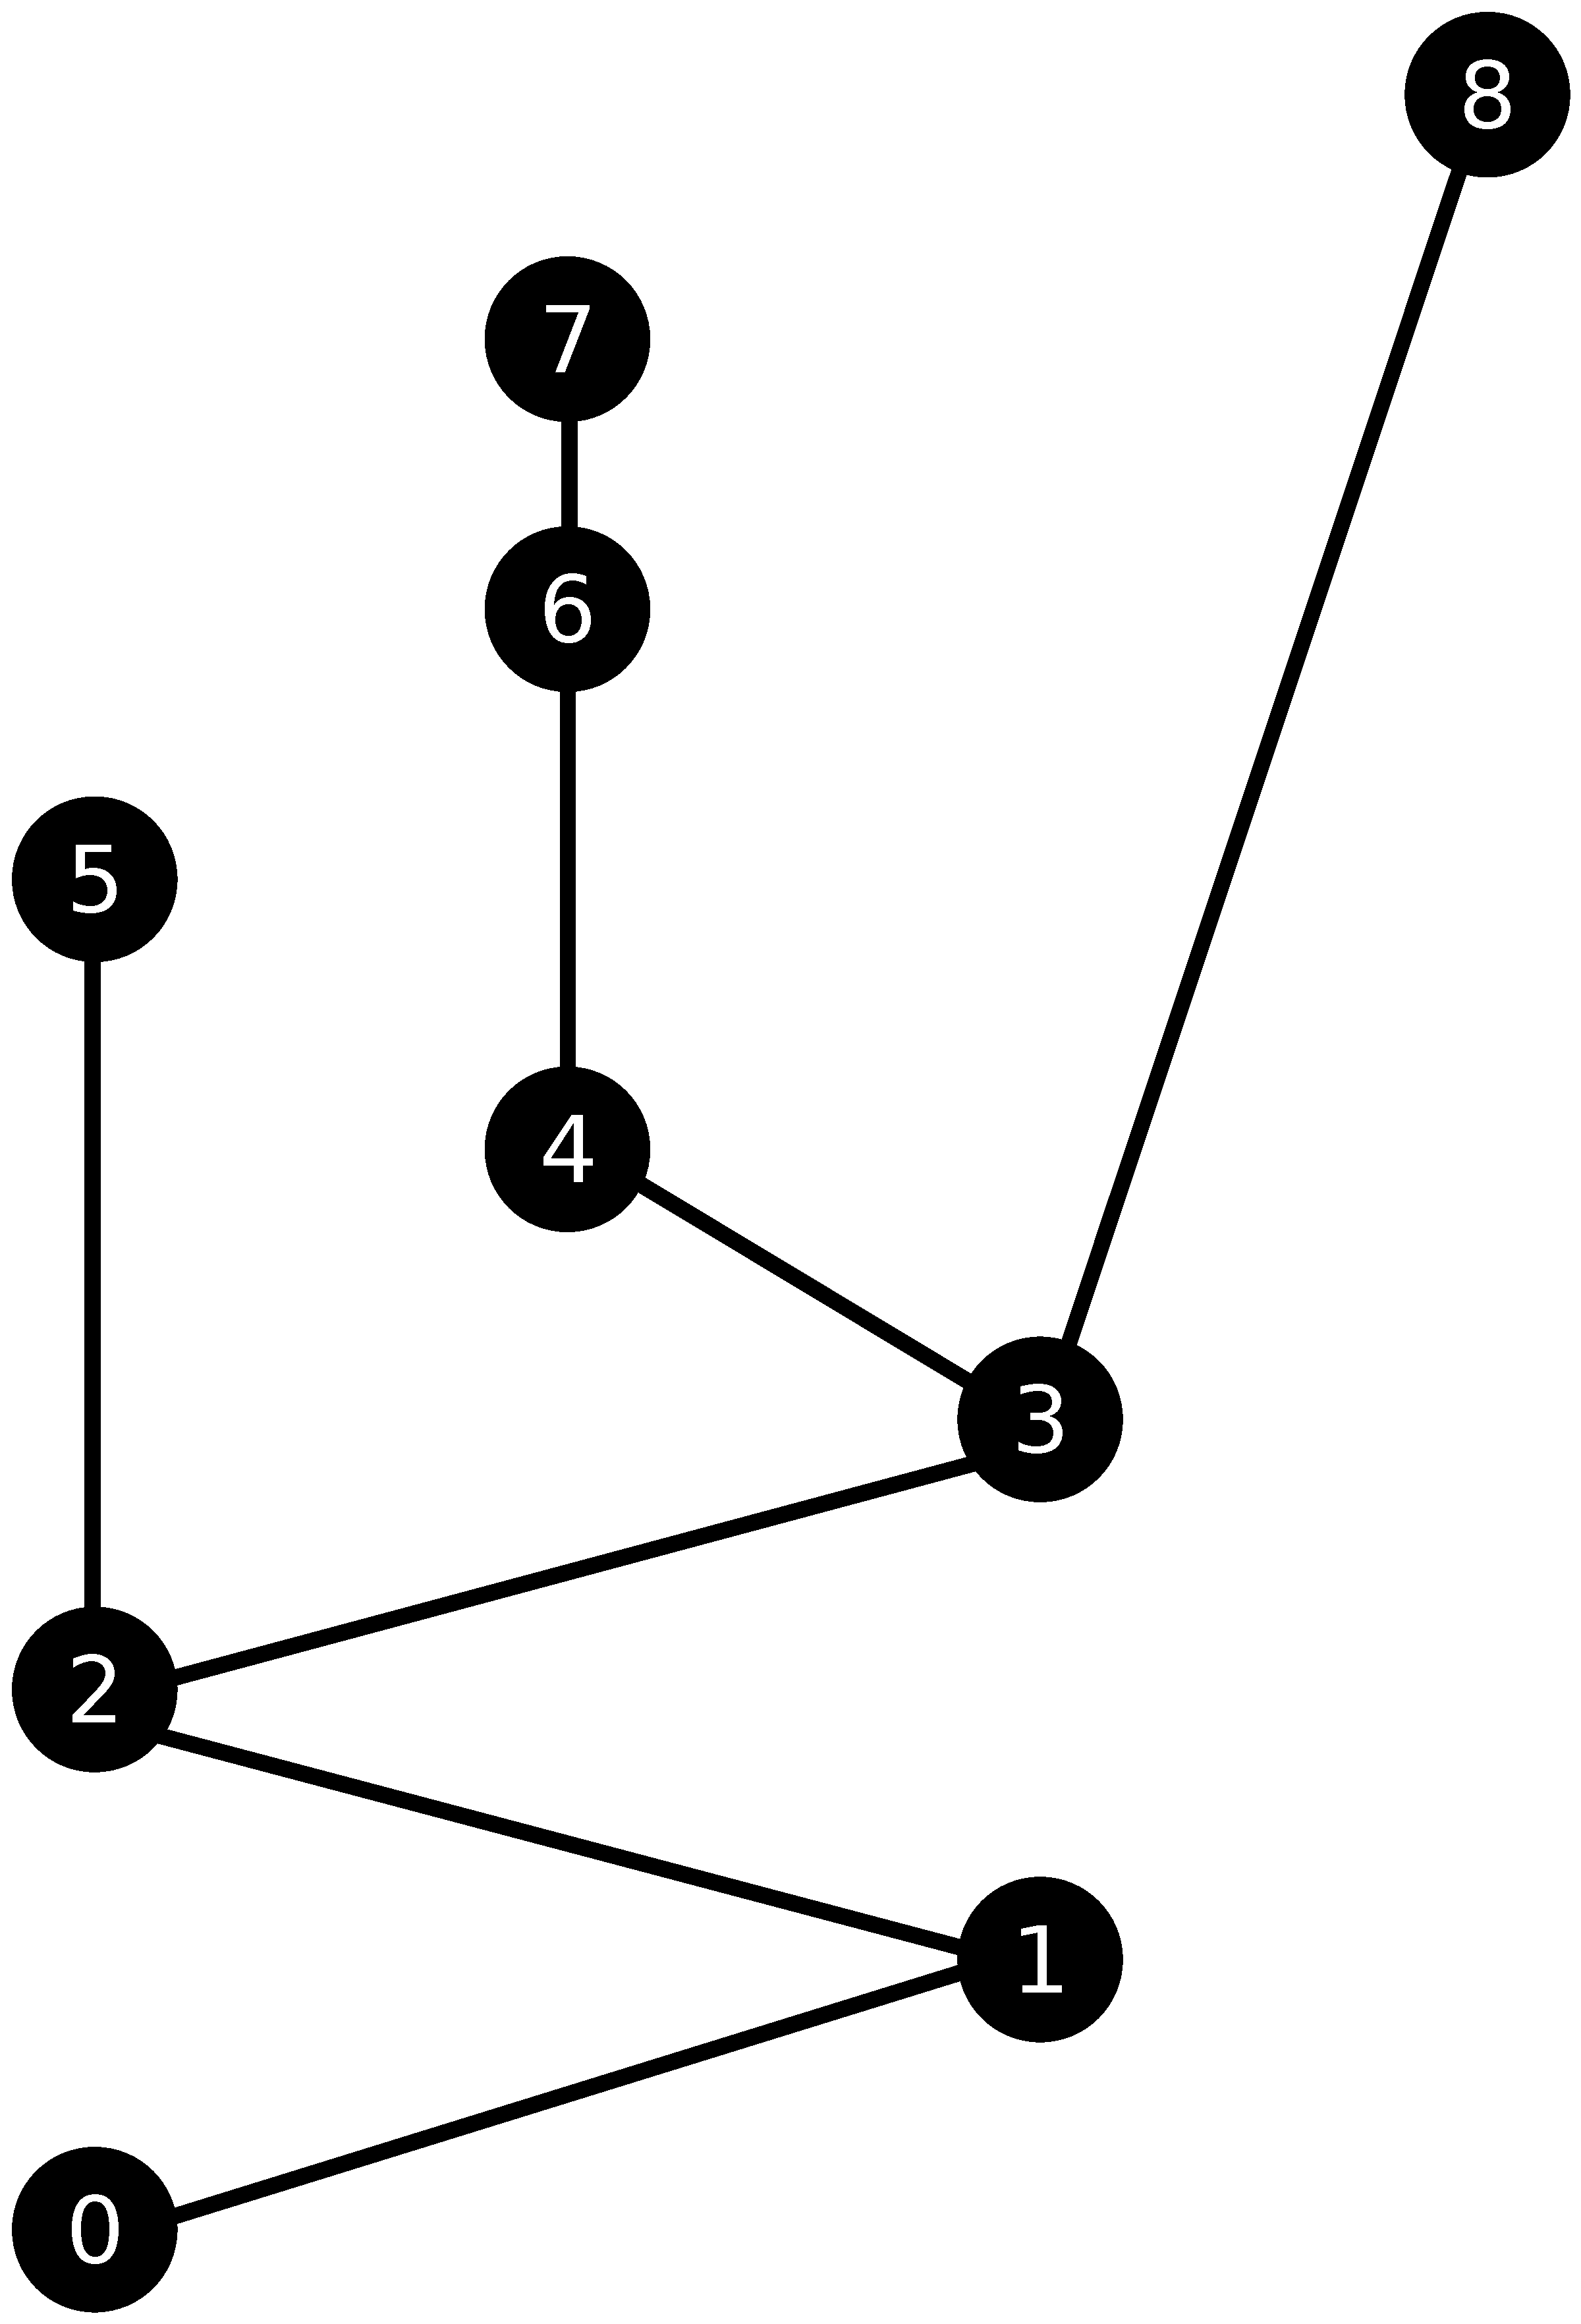
\includegraphics[scale=0.10]{./images/w3x3-join-tree-new.eps}}}%
    \qquad \qquad \qquad
    \subfloat[Split Tree]{{\includegraphics[scale=0.10]{./images/w3x3-split-tree-new.eps}}}%
    \caption{The Simplicial Mesh, Join and Split Trees and Contour Tree.}%
    \label{fig:mesh-join-split-contour}%
\end{figure}

The reason we would like to study join and split trees is that the contour tree can be reconstructed from them. The core idea of the algorithm we will present is that we can derive the join and split trees directly from the simplicial mesh and then combine them to obtain the contour tree. We will first describe how the join and split trees are computed from the mesh. We only have to describe the process for the join tree because their construction is symetrical [].

\begin{defn} A join component is a connected component in the superlevel set $f^{-1}([h, \infty))$ at some $h \in \mathbb{R}$.  \end{defn}

Let $M$ be the simplicial mesh from Figure \ref{fig:mesh-join-split-contour} (a) and let $h : M \to \mathbb{R}$ be the interpolation function defined on it. We will refer to $h$ as the height function. To construct the join tree we are going to have to keep track of which components merge together in the superlevel sets of $h$. We will consider all superlevel sets $M^t = h^{-1}([t, \infty)) = \{x \in M : h(x) \in [t, \infty) \}$ as a one parameter family $\{M^t\}_{t \in \mathbb{R}}$
of nested subsets of $M$. We can see from this definition that $M^a \subseteq M^b$ whenever $a \le b$. What the join tree captures is how the connectivity of the superlevel sets changes as the parameter $t$ is increased. The connectivity of superlevel sets changes either at local minima where a new component is created or a saddle point that merges two or more join components.

%We will not formalise the notion of tracking join components and constructing a join tree. Let us work in the general setting where $X$ is any path-connected topological space and $h : X \to \mathbb{R}$ is a function defined on $X$. The claims we make will hold in the special case where $X$ is a simplicial complex. Let us consider all sublevel sets $X_t = h^{-1}((-\infty, t]) = \{x \in X : h(x) \in (-\infty, t] \}$. They form a one parameter family $\{X_t\}_{t \in \mathbb{R}}$ of nested subsets where $X_a \subseteq X_b$ whenever $a \le b$. What the join tree captures is how the connectivity of the sublevel sets changes as the parameter $t$ is increased.

To visualise this process we can contract every join component to a point much like we did in the Reeb graph. The only difference here is that the equivalence relation is defined for all points in a superlevel set $h^{-1}([t, \infty))$ instead of a level set $h^{-1}(\{t\})$. Because of this change and because join components can only merge the join tree is a tree \cite{comp-topo}. Furthermore if $M_m = M$ is the last superlevel set for some $m \in \mathbb{R}$ then all join components merge into one because $M$ is path connected.

% @TODO Add citation

We will briefly outline the algorithm for constructing the join tree and refer the reader to \cite{ct-big-paper} for further implementational details. We know that all crical points are vertices of $M$ and that it is only at the critical points that changes in the topology of the superlevel sets can happen. The algorithm works by considering the vertices of the simplicial mesh in ascending order of their height. If the current vertex is a local minimum we directly add it in the join tree because it starts a join component. If the current vertex is a saddle that joins two or more components (join saddle) we add it to the join tree and add an edge between it and the local minima of the join components it merges. At the end of the computation all vertices will be in the same join component. In order to keep track of which join components different vertices belong to we can use the union-find data structure. The term  $\alpha(n)$ in the time complexity of the contour tree algorithm come from the basic operations of find and search in the union-find data structure.

% @TODO Define Join Saddles and Subdivided edges
Not all vertices of the mesh will be in the join tree. Only those which correspond to local maxima and to join saddles. This will pose a problem later on when we wish to combine the join and split trees. To avoid this problem we can augment the join tree by adding all missing vertices. This is done through edge subdivision. Let $a \text{ and } b$ be two adjacent vertices in the join tree.  Let $\{v_1, v_2, ..., v_n\}$ be vertices in the mesh that are not in the join tree that are given in ascending order in terms of height.  Suppose that $h(a) < h(v_i) < h(b)$ for all $i \in \{1, 2, ..., n\}$ and the vertices $v_i$ are in the same connected component of $X_b - h^{-1}(\{b\}) = h^{-1}((-\infty, b))$. In order to augment the join tree with the first vertex we subdivide the edge $ab$ and label the new vertex as $v_1$. Next we subdivide $v_1b$ and label the new vertex as $v_2$. We continue to do so and on the $k$th step we subdivide the edge
$ v_{k-1}b $ and label the new vertex as $v_k$  .

The procedure of augmentation can be applied to the split tree and contour tree as well. We can use it to augment the contour tree with all vertices of the mesh which are not critical points. This is why we will differentiate between the contour tree and the augmented contour tree. The augmented contour tree contains all regular vertices of the simplicial mesh.

The second step of the algorithm is to combine the join and split trees to produce the contour tree. We will actually combine the augmented join tree with the augmented split tree to obtain the augmented contour tree. Removing the augmentation of the contour tree is left as an optional final step. The first step in merging the two is to identify all leafs of the contour tree and their incident edges. We can recognize them immediately from the join and split trees using the following property \cite{carr-masters}.

\begin{property} Let $v$ be a vertex such that its up degree in the join tree is $0$, its down degree in the split tree is $1$ and $u$ is its only down neighbour in the split tree. Then $v$ is an up leaf in the contour tree and $vu$ is an edge in the contour tree.  \end{property}

There is an analogous property in the case of down leafs and their adjacent edges.

\begin{property} Let $v$ be a vertex such that its up degree in the join tree is $1$, its down degree in the split tree is $0$ and $u$ is its only down neighbour in the join tree. Then $v$ is a down leaf in the contour tree and $vu$ is an edge in the contour tree.  \end{property}

% @TODO Is it really known as pruning leaves?

Now suppose that we have identified $v$ as a leaf and $vu$ as its adjacent edge in the split or join tree. Another property \cite{carr-masters} tells us that if we perform vertex contraction on $v$ (remove $v$ and form a clique from its neighbourhood) from the join, split and contour trees we obtain the join and split trees of the contour tree with $v$ removed. This allows us to iteratively remove leafs from the join and split trees, add them the contour tree and them delete from the join and split tree. We can reapeat this process until we have removed all vertices from the join and split trees and all vertices are present in the contour tree. For a detailed description of this process we refer the reader to \cite{ct-big-paper}.

 % We are allowed to do so because removing all leaves in a tree leaves the tree with at least one leaf if it is not empty where the algorithm will terminate.

The Serial algorithm for the construction of the contour tree is a summary of the results we have obtained so far:

\textbf{Step 1.} Read input data and convert it to a simplicial mesh.

\textbf{Step 2.} Compute the augmented join and split trees from the simplicial mesh.

\textbf{Step 3.} Iteratively remove leafs from the augmented join and split trees and add them to the augmented contour tree until the augmented join and split trees are empty.

% @TODO Define regular vertices.
\textbf{Step 4.} Remove regular vertices from the augmented contour tree by contracting them.

\section{Parallel Algorithm}

The data parallel contour tree algorithm \cite{parallel-peak-pruning} is largely based on the serial contour tree algorithm we just described. The parallel approach borrows the two phase methodology of computing the join and split trees and then merging them. We will omit describing the process of parallelising join/split tree computation because it is not directly related to the issue we aim to address. We will describe how the merge phase is parallelised in detail.

The data-parallel paradigm works best when there are a large number of computational tasks to be carried out independently. Dependant tasks require some form of synchronisation. Synchronisation is costly in terms of performance. Removing a leaf in the merge phase of the serial algorithm requires little synchronisation with other vertices because it is a local operation. It only involves a few of the vertices of the join and split trees. This means that once we identify all up and down leafs we can remove them in parallel in a single iteration. The key problem to solve in the merge phase is to reduce the number of total iterations needed to remove all vertices from the join and split trees. The amount of parallelism in this computation is limited by the number of leafs at each iteration. For example a tree which is a path of length $n$ will take at least $n/2$ iterations and a tree with one central vertex and $n$ leafs adjacent to it will take only two iterations.

In a graph with no vertices of degree two at least half of the vertices are leafs []. If at every iterations half of the remaining vertices are leafs the total number of iterations would be logarithmic in the number of vertices in the contour tree. In order to ensure this logarithmic collapse Carr et. al \cite{parallel-peak-pruning} have come up with a way of batching some of the paths that start at a leaf and consist of vertices of degree two in a single iteration. We will call such paths leaf chains. The process of removing them in a single iteration is in effect equivalent to contracting all vertices in the tree of degree two. This leaves only leafs and vertices of degree three or higher and ensures the logarithmic collapse.

The main issue that arrises is that leaf chains which are not monotone paths are not processed in a single iteration. They require multiple iterations to process. When some of the vertices in the leaf chains have alternating height and we plot them according to height they form a characteristic zig-zag pattern. We will call paths W-Structures. See for example the path $(5, 2, 4, 3, 8)$ in the contour tree on Figure \ref{fig:mesh-join-split-contour}. These w-structures are the core issue we are addressing in this dissertation. We would like to obtain a better understanding of them and how and why they affect computation. The first step to solving such a problem is understanding it. The next chapter will address this by developing algorithms that analyse contour trees and determine the largest W-Structures that is present in them.

% The issue arises from batching monotone paths is not a monotone path and some of the vertices inside it have alternating height. The we can only batch monotone subpaths and not the whole path. The more zig zags there are in the path the less monotone paths there and the more iterations we will require. This effectively serialises computation along them.

The theoretical issue caused by the w-structures becomes evident in the algorithmic analysis of the parallel contour tree algorithm. According to that the key question in the merge phase of the algorithm is how many iterations are needed to collapse the contour tree. Each iterations takes $O(1)$ steps because all leafs can be processed in parallel and $O(t)$ work, where $t$ is the number of leaves. This leads to an overall complexity of $O(log(t))$ steps and $O(tlog^2(t)$ work if we assume that no w-structures are present. If however there is a w-structure with more "zig zags" than $log(t)$ then the authors of the paper claim that the best formal guarantee they can give for the steps is the diameter of the contour tree. One of our goals in analysing the w-structures is to provide a better bound than the diameter of the tree. We will demonstrate how this can be done by developing some new theory about the w-structures in Chapter [] and through an empirical analysis in Chapter [].


\section{Contour Tree Simplification}

Finally we will introduce the topic of contour tree simplification. A central problem in using contour trees in visualisation is simplifying their output and presenting only the most important parts to enable human comprehension. The complexity of a contour tree of a large enough data set could severly limit its use. This is why it is vital to employ techniques that simplify the contour trees by removing parts of them that correspond to less "significant" topological features or sampling noise and error. This procees helps to reveal the fundamental structures present in data.

% The most recent extensions of this work introduce high quality topological simplification [4] where the contour tree is pruned incrementally to reduce its complexity and highlight the fundamental structures present in the data.

% @TODO Add hamish phd thesis as generalisation?

One technique for contour tree simplification is branch decomposition \cite{ct-branch-decomp}. Branch decomposition involves decomposing the contour tree into a set of edge-wise disjoint monotone paths (branches) which cover all edges of the tree. The trivial branch decomposition of any tree is obtained by taking every edge to be a separate branch. A branch decomposition is hierarchical when there is exactly one branch that connects two leafs and every other branch connects a leaf to an interior node. An example of a hierarchical branch decomposition is shown in Figure \ref{fig:branch-decomp}.

The branches in this scheme represent pairs of critical points. This pairing of critical points forms the basis for a topological simplification. The topological simplification consists of removing branches that do not disconnect the tree. This produces a hierarchy of cancellations like in Figure \ref{fig:branch-decomp}. We define the persistence of a branch to be the bigger of the difference between its end points and the persistence of its children. Branches of high persistence reflect more prominent features in the tree. We apply the simplification by removing branches with low persistence that do not disconnect the tree.

The algorithm for producing the heirarchical branch decomposition of a contour tree is the following:

\begin{itemize}
    \item Identify all upper leafs that connect via branches to upwards saddles (merging of components).
    \item Identify all lower leafs that connect via branches to downwards saddles (splitting of components).
    \item Those pairs of leafs and saddles are the candidate branches. We pick the one with the lowest persistence (difference of height between the leaf and the saddle).
    \item Remove all vertices in the branch without the saddle.
    \item Continue this process untill a single branch that connect two leafs is all that remains. That is the root branch.
\end{itemize}

For example let us construct the heirarchical branch decomposition of the contour tree from Figure \ref{fig:mesh-join-split-contour}. The first two candidate branches we identify are $(5, 2)$ with persistence $3$ and $(3, 8)$ with persistence $5$. We take the branch with lower persistence $(5, 2)$. In the next step the candiate branches are $(0, 4)$ with persistence $4$ and $(3, 8)$ with persistence $5$. We will take $(0, 4)$.
Afterwards the remaining candiate branches are $(3, 7)$ with persistence $4$ and $(3, 8)$ with persistence $5$. After removing $(3, 7)$ in the final stage the only remaining branch is $(1, 8)$. It is the root branch because it connects two leafs.
The produced pairs of critical points are $(2, 5), (0, 4), (3, 7)$ and $(1,8)$.

\begin{figure}%
    \centering
    \subfloat[Branch Decomposition.]{{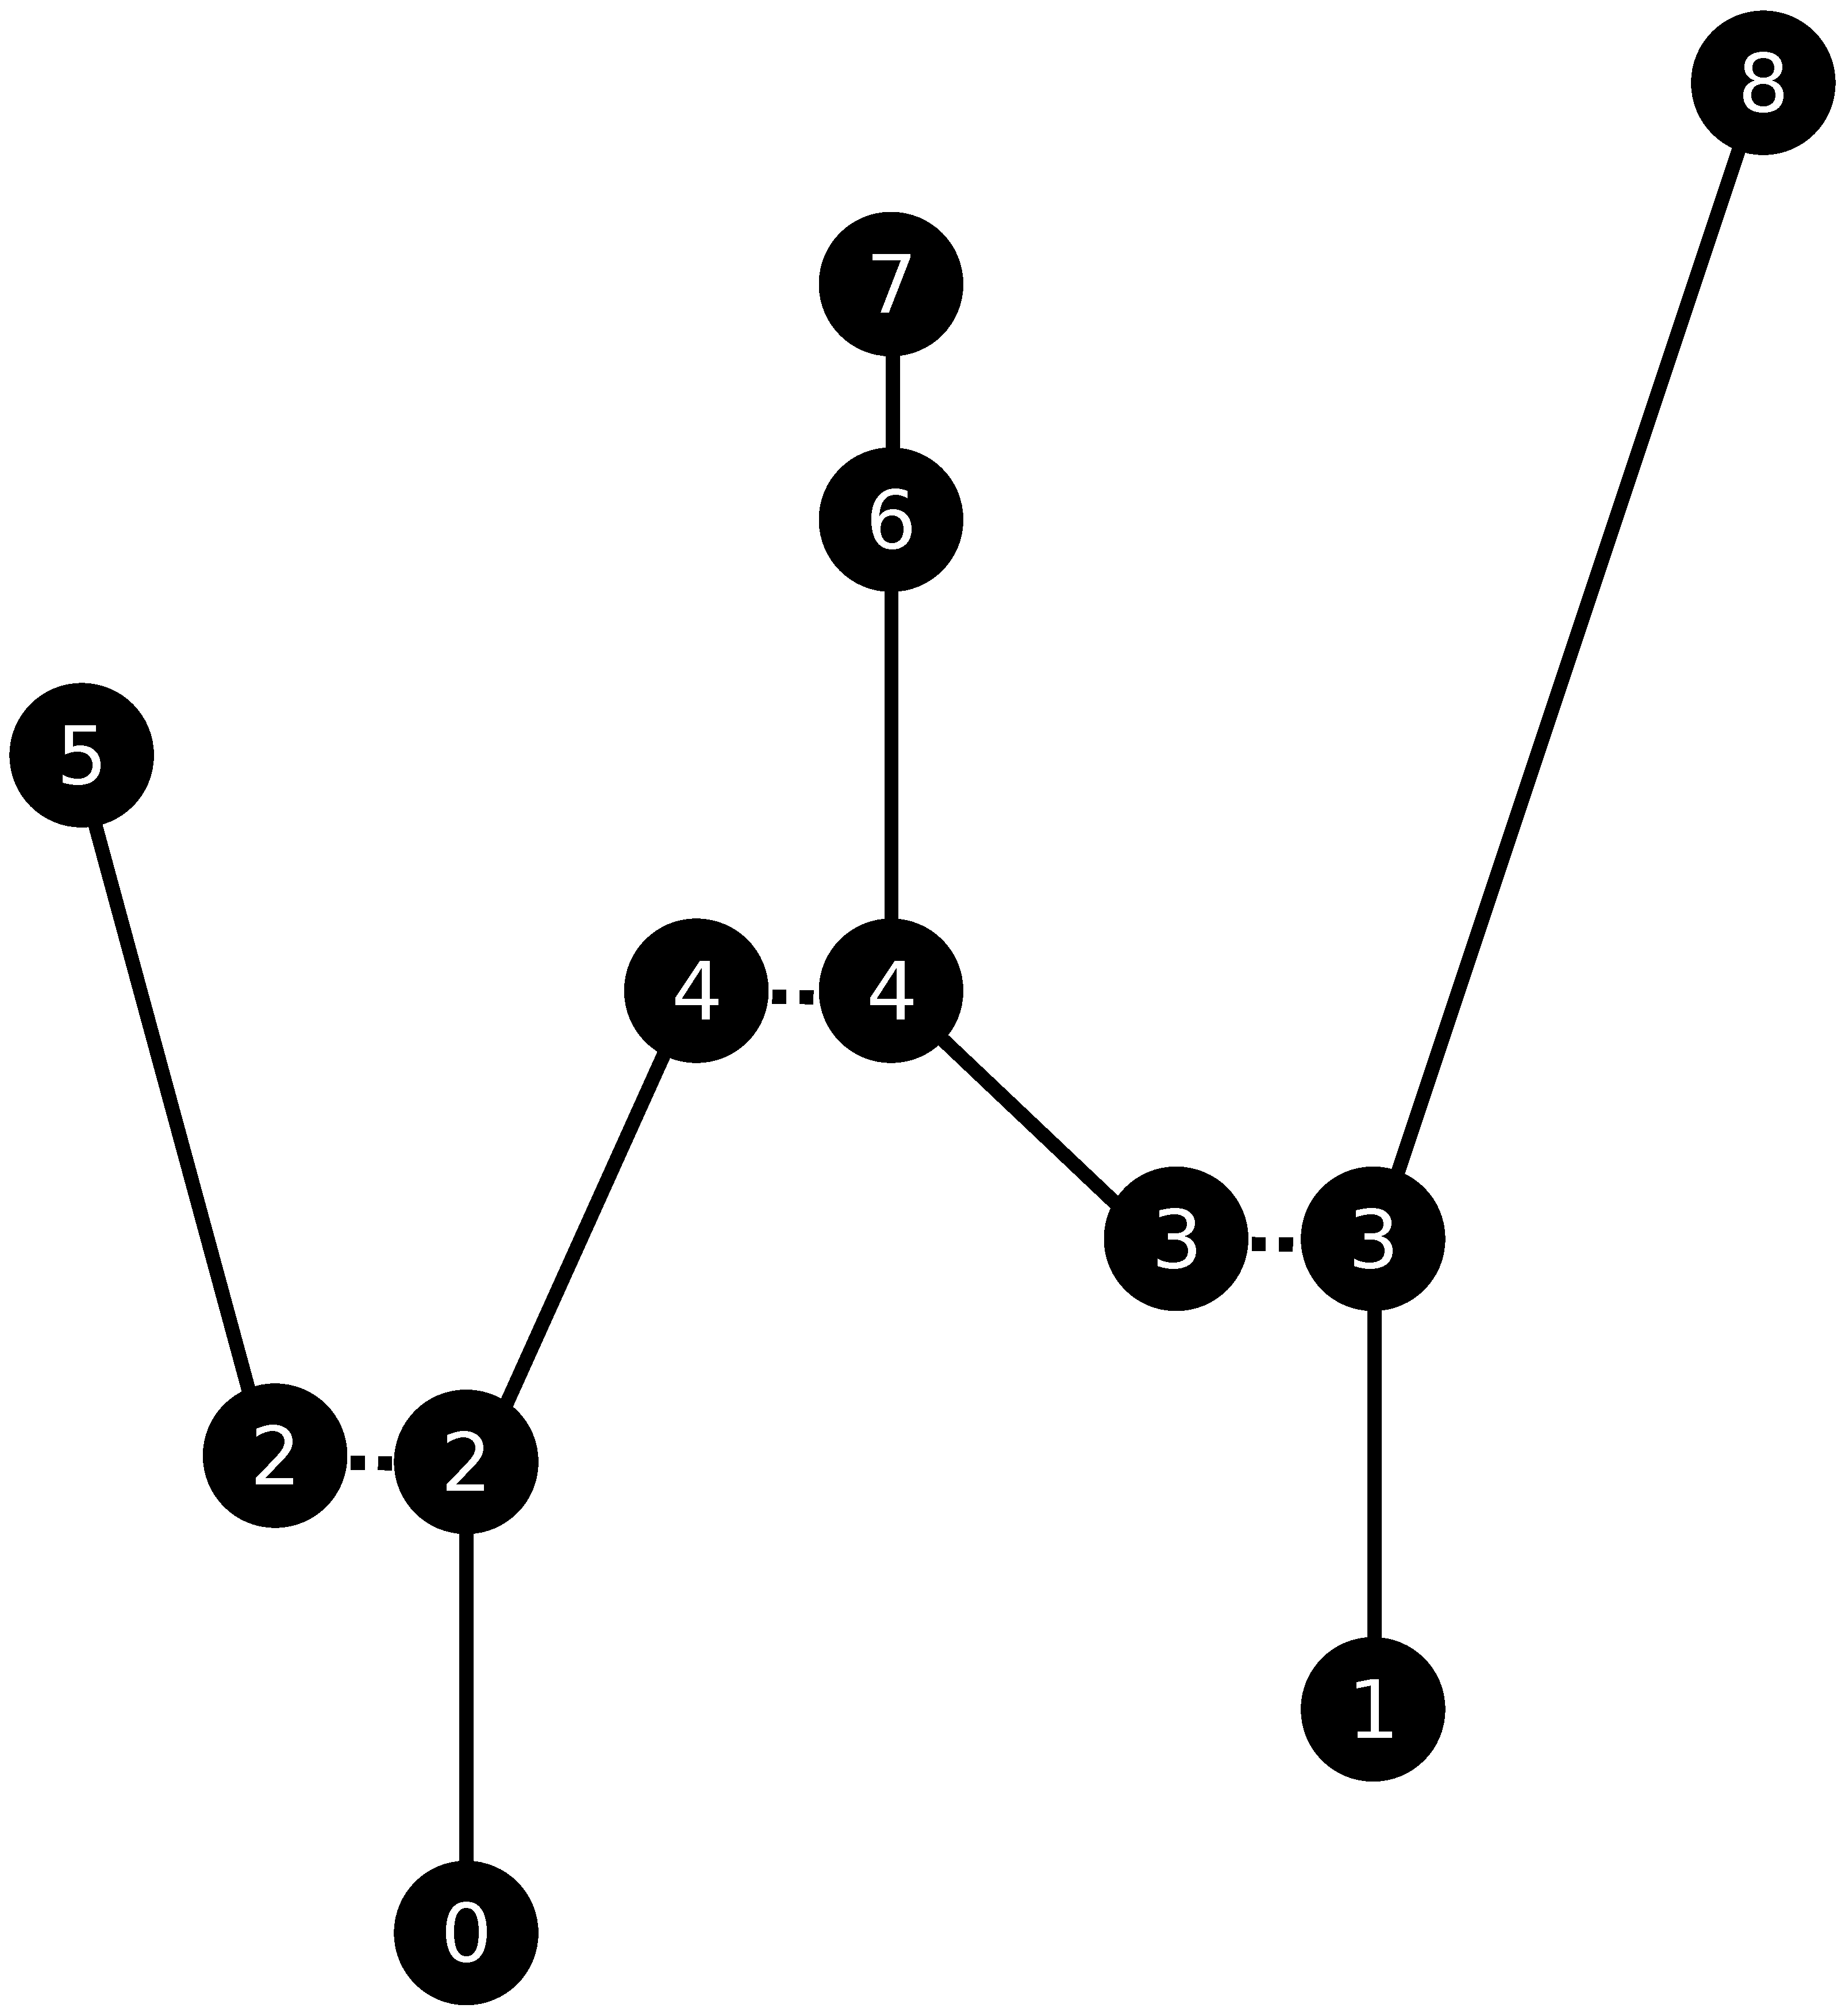
\includegraphics[scale=0.11]{./images/w3x3-ct-decomp.eps}}}%
    \subfloat[Heirarchical view of the branches.]{{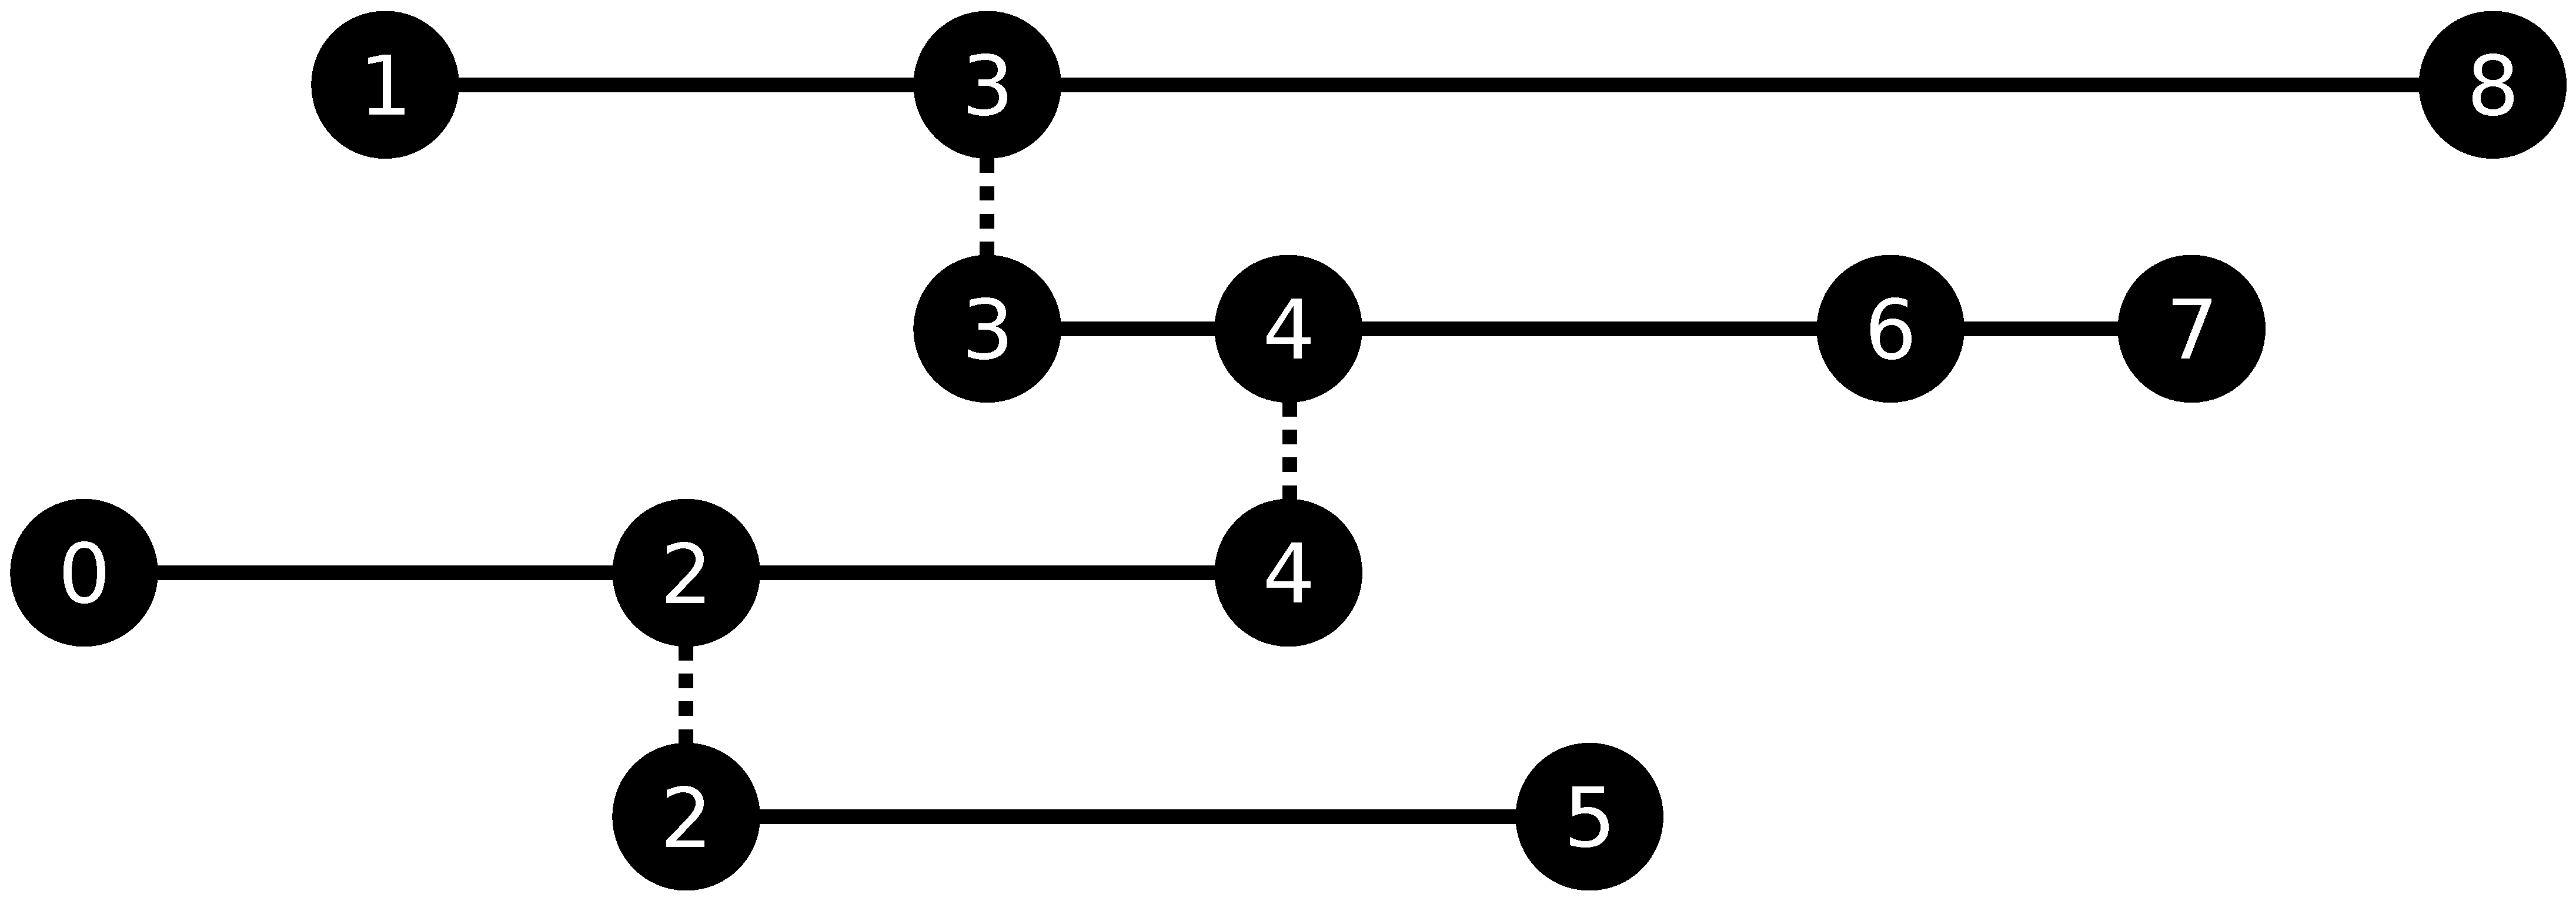
\includegraphics[scale=0.11]{./images/w3x3-ct-h-decomp.eps}}}%
    \caption{Branch Decomposition of the Contour tree from Figure \ref{fig:mesh-join-split-contour} [which subfigure?].}%
    \label{fig:branch-decomp}%
\end{figure}

Branch decomposition is a form of topological simplification whose use is limited to the contour trees. In Chapter 6 we will present a more general topological simplification framework called persistent homology. Our goal will be to express branch decomposition in the framework of persistent homology and determine whether the two are equivalent.

% @TODO Todo talk about how this is used to remove noise and artifacts in data.

% @TODO Remove Stay Tuned
% The paper \cite{ct-branch-decomp} cites that the persistence defined in that way is similar to persistence first defined in \cite{persistence-original}. In Chapter N of this dissertation we will demonstrate that this claim is either incorrect of misleading. Stay tuned folks.

% @TODO Change this
\chapter{Something "W" This Way Comes!}
\label{chapter4}

We will now continue our discussion on W-Structures in a more formal setting. In this chapter we will develop theory that captures their informal description we outlined previously. We will use it to construct three general algorithms for the detection of the largest w-structure in a height tree. We will describe the algorithms with pseudocode and provide the reader with proofs of correctness. Finally we will also demonstrate formal bounds on the time and space complexity of the proposed algorithms.

\section{Formal Description of W-Structures}

% @TODO Is this really a path definition?

We are interested in describing paths in height trees which form the characteristic zigzag pattern we described in Chapter 3. Let us first establish some of the basic notation we shall make use of. We will consider paths to be a sequence of distinct and adjacent vertices. When dealing with paths in height trees will often refer to them through their first and last vertex, because there is a unique path between any two vertices in a tree. For example when dealing with the path $v_1, v_2, v_3, v_4$ we will denote it with the shorthand $v_1 \rightsquigarrow v_4$. Lastly, a subpath of a path $P$ is a path whose vertices are also vertices of $P$.

The first important property of paths in height trees we will define is their monotone path decomposition. The monotone path decompositino of a path $P$ as a sequence of vertexwise maximal monotone subpaths of $P$ where consecutive subpaths share exactly one vertex and have alternating direction.  As shown in Figure [] $P$ can be decomposed into the sequence of paths $P_1, P_2, ..., P_k$ such that $P_i \subseteq P$, $|P_i \cap P_{i+1}| = 1$ and $P_i \cup P_{i+1}$ is not a monotone path for $i \in \{1, 2, ..., k-1\}$ and $k \ge 1$. We can use the number of paths in the monotone path decomposition to characterise paths in height trees. To simplify this characterisation note that the number of subpaths in the monotone decomposition is exactly the number of vertices in which we change direction as we traverse the path. We shall name those special vertices kinks.

%The maximum path with respect to this property is precisely the lower bound on the parallel algorithm introduced in []. As a special case we must note that paths that can be decomposed into less than four monotone paths do not pose an algorithmic problem.


A kink in a path is a vertex whose two neighbours are either both higher or both lower (Figure []). Given the path $(u_1, u_2, ... , u_k)$ an inside vertex $u_i \ne u_1, u_k$ is a kink when $h(u_i) \notin \big( min(h(u_{i-1}),~h(u_{i+1}),~max(h(u_{i-1}),~h(u_{i+1}) \big)$. To avoid this cumbersome expression we shall adopt a slight abuse of notation and in the future write it as $h(u_i) \notin $ or $ \in $ $\big(h(u_{i-1}),~h(u_{i+1}) \big)$ where it will be understood that the lower bound of the interval is the smaller of the two and the upper bound the larger.


We can use the number of kinks in a path to define a metric on it. We will call this metric the w-length of a path and use it to measure the number of inside vertices of a path which are kinks. This is similar to how the length of a path is a metric that measures the number of edges between its vertices. The notation we will adopt for the w-length and length of a path $u \rightsquigarrow u$ is $w(u, v)$ and $d(u, v)$ respectively. There is no ambiguity here because as we have already said there is a unique path between any two vertices in a tree. One thing we can already claim is that $w(u, v) \le d(u, v)$ for any two vertices in a tree. The length of a path with $n$ vertices is $n-1$, but at most $n-2$ vertices can be kinks in it.

In Chapter 3 we foreshadowed our intention of obtaining the largest W-Structure in a given contour tree. We can now put his in more precise terms as the path in a height tree that has the maximum w-length (or the longest w-path). We can immediately obtain a brute force approach for this problem by considering all paths in the height tree and computing their w-length to find the maximum one. This can be expressed with the following optimization term

$$ \max_{u, v \in V(T)}\{ w(u, v) \} .$$

The search space is quadratic in the number of vertices and measuring the w-length of a given path can be done by inspecting the height of every inside vertex and it's two neighbours in the path. The worst case running time of this algorithm is $O(d*n^2)$ where $d$ is the diameter (longest path) of the tree and $n$ is the number of vertices. This is however far from satisfactory given that the worst case time complexity of the algorithm for computing the contour tree is close to linear. We can in fact do better.

The parallel we made between the w-length and length of a path has a deeper consequences. It we were to instead ask the question of finding the longest path in a tree we would find that it is a well studied problem. Our goal now will to try to transfer that knowledge to our task at hand. We will do so by analysing how two of the most popular algorithms for computing the longest path in a tree work and whether they can be adapted to instead find the longest w-path in a tree.

%As the reader may have noticed the definitions we have made so far are analogous to the task of computing the longest path between any two vertices of a tree. This is completely intentional as we will demonstrate how algorithms for computing the longest path in a tree can be modified to produce the longest w-path instead. Finding the longest path of a graph in the general case is an \em NP-hard\em. Fortunately the Contour Tree is a tree. The longest path in a tree is known in the literature as it's diameter and has a polynomial time algorithm. The two most popular linear time algorithms found in the literature I will denote as Double Breadth First Search (2xBFS) and Dynamic Programming (DP). We will now take a look at how these algorithms work and hint at how they can be adapted in the next chapter.

\section{Tree Diameter Algorithms}

The longest path in a graph is an \em NP-hard \em problem. This can be demonstrate via a reduction to the Hamiltonian path problem []. Fortunately in the special case where the graph is a tree it has a linear time solution. In this special case it is known as the tree diameter problem. In this section we will take a look at how two of the linear time tree diameter problems work.


\subsection{Breadth First Search}

The first algorithm we will discuss is based on the following theoretical result [].

\begin{lem} Let $s$ be any vertex in a tree. Then the most distant vertex from $s$ is an endpoint of a tree diameter. \end{lem}

    To implement this algorithm we require of way of finding the most distant vertex from a given vertex. This can be done using Breadth First Search (BFS). Let $T$ be a tree and $s \in V(T)$ be any vertex. We can run BFS with $s$ as its root to find a vertex $u$ such that $d(s, u) \ge d(s, t)$ for all $t \in V(T)$. We can then run a second BFS with root $u$ to obtain a vertex $v$ such that $d(u, v) \ge d(u, t)$ for all $t \in V(T)$. As $u$ is the farthest vertex from $s$ it must be the endpoint of a diameter. As the diameter of $T$ is the longest path in $T$ therefore the second BSF must produce a path of length as much as the diameter. Therefore $d(u, v) \ge d(a, b)$ for all $a,b \in V(T)$.

The space and time complexity of BSF are linear [] and therefore the space and time complexity of this algorithm are linear as well. This follows from that fact that the algorithm consists of running BFS just two consecutive times.

\subsection{Dynamic Programming}

The second approach is based on the Dynamic Programming paradigm. Dynamic Programming is a method that is used to solve optimisation problems that exhibit recursive substructures of the same type as the original problem. The key ingredients in developing a dynamic-programming algorithm are [Into to Algorithms]:


\begin{enumerate}
    \item Characterise the structure of the optimal solution.
    \item Recursively define the value of an optimal solution.
    \item Compute the value of the optimal solution.
\end{enumerate}

% @TODO Redefine N(u)

Trees exhibit optimal substructure through their subtrees. For our intents and purposes we shall define a subtree as a connected subgraph of a tree. We will only consider rooted trees in the context of this algorithm and we must define the accordingly. Let $T$ be a rooted tree and let $v, u \in V(T)$ be two vertices such that $v$ is the parent of $u$. We shall define the subtree rooted at $u$ as the maximal (vertex-wise) subgraph of $T$ that contains $u$ but does not contain $v$.  We will denote it as $T_u$. In this notation $T = T_s$ where $s$ is the root of $T$. The rooted subtree at $u$ is smaller than $T$ as it does not contain at least one of the vertices of the $T$ namely - $v$. The structure of the optimal solution is characterised through all possible rooted subtrees $\{T_u\}_{u \in V(G)}$.

We can recursively define the value of the optimal solution with the following observation. Starting at the root of the tree the longest path in tree either goes through two children of the root and the root or is entirely contained in one of the subtrees rooted at one the children. In order to define this formally we will make use of two additional functions. Let $h(u)$ be the height of the subtree rooted at $u$. The height is defined as the longest path in $T_u$ from $u$ to one of the leaves of $T_u$. We will also define $D(u)$ as longest path contained entirely in $T_u$. The function we will maximize is $D(s)$ where $s$ is the root of $T$. We will do so with the following formula.

$$ D(v) = max\bigg\{ \max\limits_{u \in N(v)}\bigg(D(u)\bigg), \max\limits_{u, w \in N(v)}\bigg(h(u) + h(w) + 2\bigg) \bigg\}. $$

The base case for this recursive formula is at the leaves of $T$. If $u$ is a leaf of $T$ then $V(T_u) = \{u\}$. This allows us to set $h(u) = 0$ and $D(u) = 0$ and consider all leaves as base cases for the recursive formula. We are guaranteed to reach the base cases as each subtree is strictly smaller we must inevitably reach all leaves. This algorithm can be implemented in linear time using Depth First Search (DFS) by using two auxiliary arrays that hold the values for $h(u)$ and $D(u)$ for every $u \in V(T)$ []. We will elaborate more on the imeplementational details in the final section of this chapter.

%@TODO Fix sentece before

\section{Tree W-Diameter Algorithms}

%We will now step into the realm of w-detection. Before we outline the proposed algorithms we must establish two key properties which hold the difference between the tree diameter algorithms and their modification to tree w-diameter algorithms.

After introducing these two tree diameter algorithms it is now time to demonstrate how they can be adapted to the task of finding a height tree's w-diameter. Before doing so we need to establish the two key properties that will play a crutial role in adapting the algorithms.

%We have introduced two tree diameter algorithms in the previous section. Let us now demonstrate how they can be adapted to the task of computing a height tree's w-diameter. Before doing so we need to establish the two key properties that will play a critiral part in adapting the algorithms.

\begin{defn} (Subpath Property) Let $a \rightsquigarrow b$ be a path and $c \rightsquigarrow d$ its subpath. Then $w(a, b) \le w(c, d)$. \end{defn}

This property follows from the fact that all kinks of the path from $c$ to $d$ are also kinks of the path from $a$ to $b$. An important thing to note is that in the case of path length if one of the paths is a proper subpath of the other then the inequality is strict. This does not have to be the case with w-paths because the w-length decreases only when we reduce the nuber of kinks in the path.

\begin{defn} (Path Decomposition Property Property) Let $a \rightsquigarrow b$ be the path $(a, u_1, u_2, ..., u_k, b)$ and $u_i$ be an inside vertex for any $i \in \{1, 2, ..., k\}$. Then: \end{defn}

    $$w(a, b) = w(a, u_i) + w(u_i, b) + w_{a \rightsquigarrow b}(u)$$

   where:

   $$
   w_{a \rightsquigarrow b}(u_i) = \left\{
       \begin{array}{@{}l@{\thinspace}l}
           \text{0}  &: \text{if } h(u_i) \in \big(h(u_{i-1}),~h(u_{i+1}) \big) \text{ // $u_i$ is not a kink} \\
           \text{1} &: \text{otherwise // $u_i$ is a kink.} \\
       \end{array}
   \right.
   $$

We claim that $u_i$ can be a kink in the path from $a$ to $b$, but it cannot be a kink in the paths from $a$ to $u_i$ and from $u_i$ to $b$ because it is an endpoint of both. All other kinks are acounted for by either $w(a, u_i)$ or $w(u_i, b)$. Therefore when making use of path decomposition property we must account for whether the vertex we are decomposing a path at is a kink in that path or not.


\subsection{Linear Time Algorithm - 2xBFS}

Let us first explore how the Breadth First Search based tree diameter algorithm can be adapted to compute the w-diameter of a height tree. We will call the adaptation 2xBFS for short and it will follow exactly the same steps. The difference is that it will made use of a modified version of BFS that computes w-distances [see algorithm next page] from a given root vertex to all other vertices in the tree. The algorithm works by first running the modified BFS from any vertex in the graph and then records the leaf that is farthest in terms of w-length. It then runs the modified BFS a second time from that vertex and again records the farthest vertex from it. This algorihm however does is not guarateed to produce an optimal solution. It may fail to produce the tree's w-diameter, but we can bound the error in terms of the w-diameter. The correctness of the algorithm is based on the following Lemma.

\begin{algorithm}
\caption{Computing the W Diameter of a Height Tree.}

\begin{algorithmic}[1]

\Function{W\_BFS}{T, root}
    \State root.d = 0
    \State root.$\pi$ = root
    \State furthest = root

    \State Q = $\emptyset$
    \State Enqueue(Q, root)

    \While {Q $\ne \emptyset$}
        \State u = Dequeue(Q)

        \If {u.d $>$ furthest.d}
            \State furthest = u
        \EndIf

        \ForAll {v $\in$ T.$Adj$[u]}
            \If {v.$\pi$ == $\emptyset$}
                \State v.$\pi$ = u
                \If {h(u) $\notin$ \big(h(v),~h(u.$\pi$)\big)}
                    \State v.d = u.d + 1
                \Else
                    \State v.d = u.d
                \EndIf

                \State Enqueue(Q, v)

            \EndIf
        \EndFor
    \EndWhile
    \State Return furthest
\EndFunction

\Function{Calculate\_W\_Diameter}{T}
    \State s = <any vertex>
    \State u = W\_BFS(T, s)
    \State v = W\_BFS(T, u)
    \State return v.d
\EndFunction

\end{algorithmic}
\end{algorithm}



%\begin{lem} The Algorithm produces the endpoints of a path who is at most 2 kinks shy of being the kinkiest path in the tree. \end{lem}

\begin{lem} The farthest leaf in terms of w-length from any vertex in a height tree is guaranteed to be the endpoint of a path in the tree whose w-length is at least that of the w-diameter of the tree minus two. \end{lem}



\begin{proof}
Let $T$ be a height tree and $s \in V(T)$ be the initial vertex we start the first search at. After running the modified BFS twice we obtain two vertices $u$ and $v$ such that:

\begin{equation}
    \label{eq:su_all}
    w(s, u) \ge w(s, t), \forall t \in V(T)
\end{equation}

\begin{equation}
    \label{eq:uv_all}
    w(u, v) \ge w(u, t), \forall t \in V(T).
\end{equation}

Furthermore let $a$ and $b$ be two leaves that are the endpoints of a path that is a w-diameter. For any such pair we know that:

\begin{equation}
    \label{eq:ab_all}
    w(a, b) \ge w(c, d), \forall c, d \in V(T)
\end{equation}

By this equation we have that $w(a, b) \ge w(u, v)$. Our goal in this proof will be to give a formal lower bound on $w(u, v)$ in terms of $w(a, b)$. To this end let $t$ be the first vertex in the path between $a$ and $b$ that the first BFS starting at $s$ discovers. We can infer that $t$ cannot be $a$ or $b$ unless $s$ is equal to $a$ or $b$.

The proof can then be split into several cases depending on the relative positions of $s$, $t$, $a$, $b$ and $u$. \linebreak

{\em Case 1. When the path from $a$ to $b$ does not share any vertices with the path from $s$ to $u$.}

{\em Case 1.1. When the path from $u$ to $t$ goes through $s$.}



% @TODO Explain that the dotted lines are paths.
\begin{figure}%
    \centering
    \includegraphics[center, scale=0.5 ]{./images/2xbfs-case-1-1.eps}
    \caption{Relative position of vertices in Case 1.1 }%
    \label{fig:case1.1}%
\end{figure}

In this case $s \rightsquigarrow u$ is a subpath of $t \rightsquigarrow u$, which in turn means that $w(t, u) \ge w(s, u)$. By equation \ref{eq:uv_all} we also have that $w(s, u) \ge w(s, a)$. We can therefore conclude that $w(t, u) \ge w(a, t)$ as $s \rightsquigarrow a$ is a subpath of $t \rightsquigarrow a$.

Now via path decomposition of $a \rightsquigarrow b$ and $u \rightsquigarrow b$ at $t$ have that:

$$ w(a, b) = w(b, t) + w(t, a) + x  $$
$$ w(u, b) = w(b, t) + w(t, u) + y .$$

Where $x, y \in \{0, 1\}$ depending on whether there is a kink at $t$ for the path from $a$ to $b$ and from $u$ to $b$ respectively. As $w(t, u) \ge w(a, t)$ we can show that:


$$ w(u, b) \ge w(b, t) + w(t, a) + y $$
$$ w(u, b) \ge w(b, t) + w(t, a) + x - x + y $$
$$ w(u, b) \ge w(a, b) - x + y $$
$$ w(u, b) \ge w(a, b) + (y - x) $$

But as $w(u, v) \ge w(u, b)$ (by equation \ref{eq:uv_all}) we obtain that: Sha
$$ w(u, v) \ge w(a, b) + (y - x) $$

Considering all possible values that $x$ and $y$ can take, we can see that the minimum value for the right hand side of the inequality is at $y = 0$ and $x = 1$. The final conclusion we may draw is that $w(u, v) \ge w(a, b) -1$.



%$a\rightsquigarrow b$

{\em Case 1.2. When the path from $u$ to $t$ does not go through $s$.}

\begin{figure}%
    \centering
    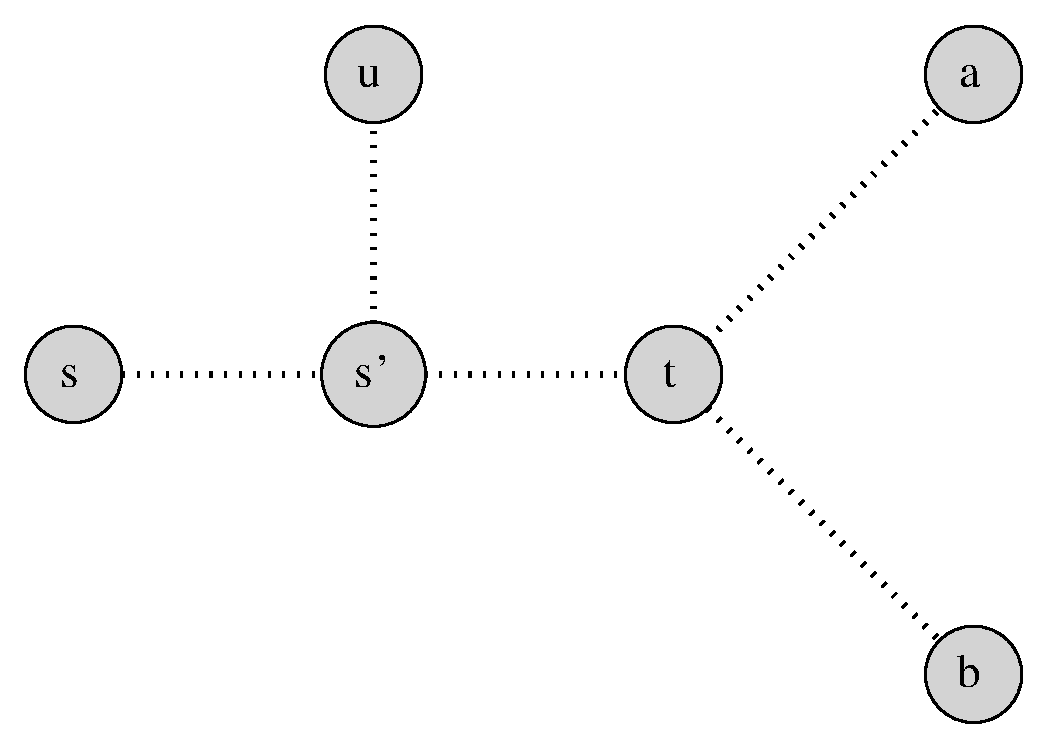
\includegraphics[center, scale=0.5 ]{./images/2xbfs-case-1-2.eps}
    \caption{Relative position of vertices in Case 1.2 }%
    \label{fig:case1.2}%
\end{figure}

If the path from $u$ to $t$ does not go through $s$ then the paths $s \rightsquigarrow t$ and $s \rightsquigarrow u$ have a common subpath. Let $s'$ be the last common vertex in that subpath. We will be able to produce s proof that is similar to the previous case by considering $s'$ in the place of $s$. We must only account for whether $s'$ is a kink in one of the paths $s \rightsquigarrow u$ or $s \rightsquigarrow t$. We know that $w(t, u) \ge w(s', u)$ (as a subpath) and through path decomposition of  $s \rightsquigarrow a$ and $s \rightsquigarrow u$ at $s'$ we obtain that:

$$ w(s, a) = w(s, s') + w(s', a) + x $$
$$ w(s, u) = w(s, s') + w(s', u) + y $$

where $x,y \in \{0, 1\}$ indicate whether $s'$ is a kink in the corresponding path as before. By equation \ref{eq:su_all} we know that $w(s, u) \ge w(s, a)$ and therefore:

$$ w(s, s') + w(s', u) + y \ge w(s, s') + w(s', a) + x  $$
$$ w(s', u) + y \ge w(s', a) + x $$
$$ w(s', u) \ge w(s', a) + (x - y).$$

Since $s'$ lies on the path from $t$ to $u$ we have that $w(t, u) \ge w(s', u)$ by the subpath property. We can use this to conclude the following:

$$ w(t, u) \ge w(s', a) + (x - y).$$

From the fact that $t \rightsquigarrow a$ is a subpath of $s' \rightsquigarrow a$ it follows that $w(s', a) \ge w(t, a)$. This allows us to infer that:

$$ w(t, u) \ge w(t, a) + (x - y). $$

Now we are ready to proceed in a similar manner as the previous case. We will decompose the paths from $b$ to $a$ and from $b$ to $u$ at the vertex $t$ as follows:

$$ w(b, a) = w(b, t) + w(t, a) + z  $$
$$ w(b, u) = w(b, t) + w(t, u) + w  $$
$$ w(b, u) \ge w(b, t) + w(t, a) + (x - y) + w $$
$$ w(b, u) \ge w(b, t) + w(t, a) + z - z + (x - y) + w $$
$$ w(b, u) \ge w(a, b) - z + (x - y) + w $$
$$ w(b, u) \ge w(a, b) + (x - y) + (w - z) $$

The minimum value for the right hand side of this equation is at $x, w = 0$ and $y, z = 1$. Using the fact that $w(u, v) \ge w(u, b)$ we finally obtain $ w(u, v) \ge w(a, b) - 2 $.


{\em Case 2. When the path from $a$ to $b$ shares at least one vertex with the path from $s$ to $u$.}

\begin{figure}%
    \centering
    \includegraphics[center, scale=0.5 ]{./images/2xbfs-case-2.eps}
    \caption{Relative position of vertices in Case 2 ($t$ could be equal to $s'$). }%
    \label{fig:case2}%
\end{figure}

% @TODO This is not complete!
%As we already know $w(s, u) \ge w(s, a)$. Furthermore $w(s, u) \ge w(t, u)$ and $w(s, a) \ge w(t, a)$ as they are subpaths of $s \rightsquigarrow u$ and $s \rightsquigarrow a$ respectively. Therefore $w(t, u) \ge w(t, a)$. We can now decompose the paths from $b$ to $a$ and from $b$ to $u$ at the vertex $t$ as follows:

We can do a path decomposition as follows:

$$ w(s, u) = w(s, t) + w(t, u) + x $$
$$ w(s, a) = w(s, t) + w(t, a) + y $$

As $w(s, u) \ge w(s, a)$ (by equation \ref{eq:uv_all})we obtain that:

$$ w(s, t) + w(t, u) + x  \ge w(s, t) + w(t, a) + y $$
$$ w(t, u) \ge w(t, a) + (y - x) $$

If we again decompose the paths from $b$ to $a$ and from $b$ to $u$ at $t$ we obtain:

$$ w(b, a) = w(b, t) + w(t, a) + z  $$
$$ w(b, u) = w(b, t) + w(t, u) + w  $$
$$ w(b, u) \ge w(b, t) + w(t, a) + (x - y) + w $$
$$ w(b, u) \ge (w(b, t) + w(t, a) + z) - z + (x - y) + w $$
$$ w(b, u) \ge w(a, b) - z (x - y) + w $$
$$ w(b, u) \ge w(a, b) + (x - y) + (w - z). $$

Where similarly to the previous case the rightful conclusion is that $ w(u, v) \ge w(a, b) - 2 $.

Based on these cases we can have shown that that for any input tree the algorithm will produce a w-path that is at most two kinks less than the actual maximum w-path.


\end{proof}

Let us now show some formal bounds on the time and space complexity of the 2xBFS algorithm.

\begin{lem} The time complexity of the algorithm is $O(|V|)$. \end{lem}

\begin{proof}
    The modified BFS function has the same time complexity as BFS. All we have added to the standard BFS is an "\em if, then, else\em"~statement. The time complexity of BFS is $O(|V| + |E|)$, but in a tree $|E| = |V| - 1$, so the overall complexity is $O(2|V| - 1) = O(|V|)$.
    Running the modified BFS function a second time only adds a linear factor the expression and thus the overall complexity of the algorithm is linear.
\end{proof}

\begin{lem} The space complexity of the algorithm is $O(|V|)$. \end{lem}

\begin{proof}
    The modified BFS function has the same memory complexity as the standard BFS. Therefore the space complexity of 2xBFS is $O(|V|)$.
\end{proof}

\subsection{Pathological Cases in 2xBFS}

Here we will present some examples of pathological cases where the w-diameter outputted by the 2xBFS algorithm differs from the actual w-diameter (Figure \ref{fig:path-cases}). Each one of the examples corresponds to one of the cases in Lemma []. In all examples the initial vertex is taked to be $s$. After running the algorithm we can see that the vertex outputted by the first BFS function would be $u$ after which the longest path would be outputted as $u \rightsquigarrow a$ or $u \rightsquigarrow b$. We can see that that in all figures $w(u, a) = w(u, b) = 1 \text{ or } 2$, but $w(a, b) = 3$.

Even if we adapt the algorithm so that it finds the vertex with that is farthest in terms of both w-length and length we will still be able to make simillar pathological case examples. We just need to augment the height trees by making $u$ further away from $s$ that $a$ and $b$ but keeping the same relative w-length of all paths.

\begin{figure}%
    \centering

    \subfloat[Pathological Example for Case 1. 1 (-1 of actual w-diameter).]{{\includegraphics[scale=0.4]{./images/2xbfs-path-case-1-1.eps}}}%
    \qquad
    \subfloat[Pathological Example for Case 1. 2 (-2 of actual w-diameter).]{{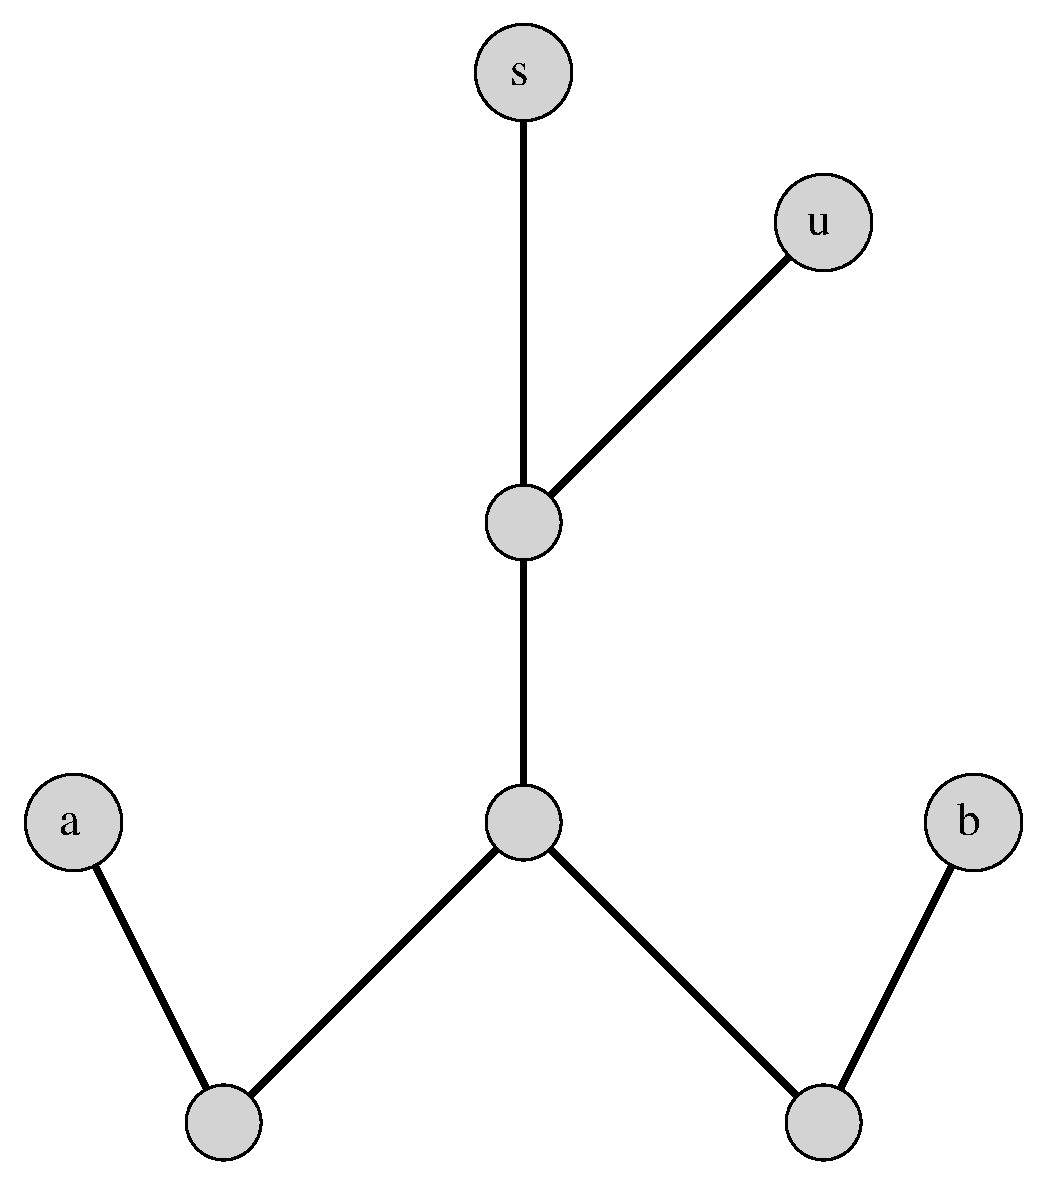
\includegraphics[scale=0.4 ]{./images/2xbfs-path-case-1-2.eps}}}%
    \qquad
    \subfloat[Pathological Example for Case 2 (-2 of actual 2-diameter).]{{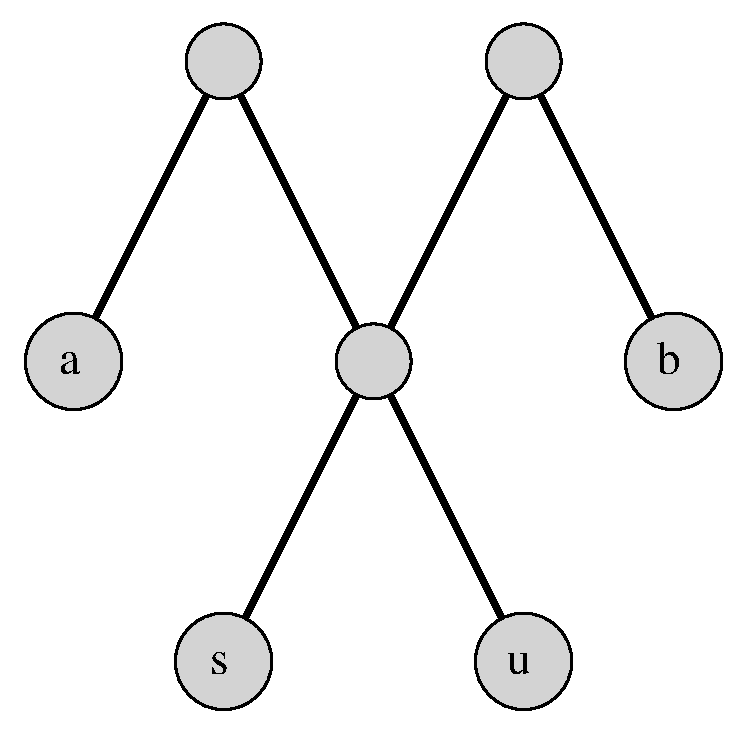
\includegraphics[scale=0.6 ]{./images/2xbfs-path-case-2.eps}}}%
    \caption{Branch Decomposition of a Contour tree.}%
    \label{fig:path-cases}%
\end{figure}



\subsection{Attempts at resolving the accuracy of 2xBFS}


% @TODO Chapter 3 here may change.

%For the intents and purposes of this dissertation the accuracy of this algorithm is sufficient. In large enough data sets this estimate provides enough insight to correlate the observed iterations needed to collapse the split and join trees and the resulting w-diameter of the tree. This is demonstrated empirically in Chapter 3. Regardless of such practical considerations it is still of inherent theoretical interest to investigate how we may be able to obtain a more accurate modification of this algorithm.

In this section we adapted the first of the tree diameter algorithms to obtain a w-diameter algorithm with what we claim is reasonable accurate. That accuracy is supported by Lemma [], but we have not way of knowing whether the w-path obtained through 2xBFS is optimal of not. Here we will present two possible ways of improving the accuracy of the output of the 2xBFS algorithm and explain why were not able improve upon the theoretical bound of Lemma [].

One key observation we can make is that on the second run of the BFS we get a w-path that is necessarily longer or equal to one found in the first BFS search. A natural question to ask is whether running the BFS a third, fourth or for that matter nth time would result in the actual w-diameter. On every successive iteration we get a w-path that is longer or equal to the previous one, because w-length is a symmetric path property ($w(a, b) = w(b, a)$). By doing this we can hope that we will eventually obtain a w-path closer to the w-diameter. However there is no guarantee that this will happen. In some cases it is possible that each successive BFS returns the same path over and over again. Obverse how in Figure [] all iterations of BFS go from the vertex $u$ to the vertex $v$ and then from $v$ to $u$ and so on.

A different heuristic we can apply is to run the algorithm multiple times from different starting vertices and keep the maximum value found. This approach is more reliable for if we run the algorithm from all vertices in the tree we will obtain the actual w-diameter. The ussue in doing is that the time complexity will become quadratic and we would be no better off that with the exhaustive brute force approach. If however we run the algorithm for some subset of the vertices in the tree we lose all guaratees on the accuracy. There may simply be too few vertices from which the algorithm would obtain the actual w-diameter.

%Consider @TODO fig[]. That artificial example shows that there can simply be too few starting points which would produce the w-diameter.


% @TODO Redo Last Paragraph.
%In the search for a better solution let $s$ be a starting vertex and let the vertices $U = \{u_1, u_2, ..., u_n\}$ be the furthest away in terms of w-distance and $W = \{w_1, w_2, ..., w_n\}$ be the ones second furthest away. By the proof of the algorithm we know that not necessarily all vertices in those sets would produce a w-diameter. Thus lets us define $R \subseteq U \cup W$ as the set of vertices which are endpoints of a w-diameter. As we have shown we can construct an example where $|R| = 2$ and $|U \cup W|$ is arbitrarily large. Can we then find some property of the vertices in $R$ and pick them out in the first phase of the algorithm? *This I will leave open for the future generations to ponder. I hope in doing so all people of the world will unite unite and end all wars and prejudices in order to work towards this common good!*

\subsection{Dynamic Programming Algorithm - DP}

% @TODO
%*Idea redefine $N(u) = N(u) / u.\pi$ so you can simplify notation.*

It is encouraging that we have obtained an algorithm that bounds the w-diameter but it is also unsatisfactory that we were not able to directly obtain it. To remedy this we will resort to modifying the second tree diameter algorithm that we outlined previously. We will use the same optimisation strategy i.e. dynamic programming by making two key changes. Instead of the function $h(u)$ that computes the height of a subtree with root $u$ we will use the function $w(u)$ that stores the longest w-path that starts at the root of the subtree. We will remane the function that stores the value of the optimal solution for subroblems from $D(u)$ to $W(u)$ accordingly. To summarise $W(u)$ returns the length of the largest w-path in the subtree $T_u$ and $w(u)$ the length of the largest w-path in $T_u$ that starts at $u$.

%This may seem like a simple substitution at first glance, but the devil is in the details.
Similarly to the modification of the BFS based algorithm all additional difficulties stem from the difference in the properties of length and w-legnth of paths. Let us first define the w-height of rooted height tree. It is the longest w-path that starts at the root of the tree. We will now examine how w-height can be computed in manner similar to the height of a rooted tree. Let $T$ be a rooted tree and $s \in V(T)$ be any vertex. Let us also assume the we have computed the w-heights of the children of $s$. In the case of computing the height we can simply set $h(s) = \max\limits_{u \in N(s)}\big( h(u) \big) + 1$. We cannot do so with the w-height because w-length can remain the same if we do not extend the maximum w-path with a kink.  To demonstrate this let us assume that $u \in N(s)$ is such that $w(u) = \max\limits_{v \in N(s)}(w(v))$. Then if we wish to extend the maximum w-path that ends at $u$ to $s$ we must account for whether $u$ becomes a kink in it. If none of the children of $s$ with maximum w-height form a kink when extending to $s$ then the w-height of $s$ does not increase.

In order to obtain the w-height of $s$ let $u$ be any of it's children and $L_u = \{u_1, u_2, ..., u_k\}$ be all children of $u$ through which a w-path with length $w(u)$ passes through. We can compute the w-height of $s$ as follows: $w(s) = \max\limits_{u \in N(s)}\{ h(u) + \max\limits_{v \in L_u}(w_{s \rightsquigarrow v}(u)) \}$. In other words there may be multiple w-paths with the same maximal w-length that end at $u$. If possible we must pick the one that would make $u$ form a kink with $s$. If not we can use any of them. It is of no use to consider paths of lesser w-length because when adding $s$ to them the w-length may increase by at most one and match any of the paths that end in $L_u$.

The second ingredient in the dynamic programming approach of the tree diameter algorithm was to combine the two longest paths that end at children of the root of the subtree. As before let $T$ be a tree and $s$ be its root. We first find two distinct children $u, v \in N(s)$ of $s$ such that $h(u)$ and $h(v)$ is maximum amongst all children and $u \ne v$ (otherwise we do not get a proper path). Next we will combine the longest paths and at $u$ and $v$ in order to obtain the longest path that goes through $s$. The length of this new path is given by the summation $h(u) + h(v) + 2$. The $2$ is added to account for the two additional edges $us, sv \in E(T_s)$. This method of combinig paths extends of course extends to all subtrees in $T$.

In the case of w-path combinations we must be vigilant of which vertices become kinks in the path combinations. Let us observe a similar scenario where $s$ is the root a rooted tree $T$ and $u, v \in V(T_s)$ are two of the children with maximal values for $w(u)$ and $w(v)$. We would ideally like to combine $w(u)$ and $w(v)$ like so: $w(u) + w(v) + w_{u, v}(s)$. This however is not correct! There is a hidden assumption in the sum that the only vertex that can become a kink in this path combination is $s$. Contrary to this, in fact $u$ and $v$ can also become kinks. Observe that $w(u) \text{ and } w(v)$ are the w-lengths of two paths. One path starting at $u$ and ending in a leaf of $T_u$ and one starting at $v$ and ending in a leaf of $T_v$. In the new path both $u$ and $v$ become inside vertices and depending on whether they become kinks or not the sum may further increase by two. To account for this we must also look at the children of $u$ and $v$ through which a maximum w-path passes. We have already introduced those as $L_u$ and $L_v$. This process is similar to the one for obtaining the w-height of a vertex and is described by the following formula:

$$ w(u) = \max\limits_{\substack{u, v \in N(s) \\ u \ne v}}\{ h(u) + \max\limits_{t \in L_u}\Big(w_{s \rightsquigarrow t}(u)\Big) + h(v) + \max\limits_{t \in L_v}\Big(w_{s \rightsquigarrow t}(v)\Big) + w_{u \rightsquigarrow v}(s)\}. $$

%Thus the formula that describes the optimal solution can be written as:

We now claim that the longest w-path in a rooted height tree is either entirely contained in one of the subtrees of the root or is a combination of two maximum w-height paths that end at two distinct children of the root. Combining what we have shows so far we obtain the following expression for the optimal solution:

$$ W(s) = max\Bigg\{ \max\limits_{u \in N(s)}\bigg(W(u)\bigg), \max\limits_{\substack{u, v \in N(s) \\ u \ne v}} \bigg( h(u) + \max\limits_{t \in L_u}\Big(w_{s \rightsquigarrow t}(u)\Big) + h(v) + \max\limits_{t \in L_v}\Big(w_{s \rightsquigarrow t}(v)\Big) + w_{u \rightsquigarrow v}(s) \bigg) \Bigg\}. $$

Here is the pseudocode for a recursive implementation of this algorithm.


\begin{algorithm}{}
\caption{Computing the W Diameter of a Height Tree.}
\begin{algorithmic}[1]

%\Function{W\_DFS}{T, s}
    \State{\textbf{Function}W\_DFS}(T, s)

    % If we are at a leaf Base Case
    \State // Base Case
    \If {|T.$Adj$[s]| == 1 AND s.$\pi \ne $ s}
        \State s.W = 0
        \State s.w = 0
        \State return
    \EndIf

    % Forwards DFS visit

    \State // DFS Visit
    \ForAll {u $\in$ T.$Adj$[s]}
        \If {u.$\pi$ == $\emptyset$}
            \State u.$\pi$ = s
            \State W\_DFS(T, u)
        \EndIf
    \EndFor

    % Backtracking
    \\

    \State // After all neighbours are visited

    \State // Calculate w-height of s
    \ForAll {u $\in$ T.$Adj$[s]$/s.\pi$}
        \If {L[u] == $\emptyset$}
            \State H[s] = max(H[s], H[u]);
        \Else
            \ForAll {v $\in$ L[u]$/u$}
                \State H[s] = max(H[s], H[u] + $w_{v, s}(u)$);
            \EndFor
        \EndIf
    \EndFor

    \State // Find all children that contribute to the a w-height path
    \ForAll {u $\in$ T.$Adj$[s]$/s.\pi$}
        \If {L[u] == $\emptyset$ AND H[s] == H[u]}
            \State L[s] = L[s] $\cup$ u
        \Else
            \ForAll {v $\in$ L[u]$/u$}
                \If {H[s] = max(H[s], H[u] + $w_{v, s}(u)$)}
                    \State L[s] = L[s] $\cup$ u
                \EndIf
            \EndFor
        \EndIf
    \EndFor

    \State // Find the maximum path combination
    \State maxCombine = 0
    \ForAll {u $\in$ T.$Adj$[s]$/s.\pi$}

        \ForAll {v $\in$ T.$Adj$[s]$/s.\pi$}

            \If {v == u}
                \State continue
            \EndIf

            \State temp = H[u] + H[v]

            \If {L[u] $\ne$ $\emptyset$}
                \ForAll {t $\in$ L[u]$/u$}
                    \If {$w_{t, s}(u) == 1$}
                        \State temp = temp + 1
                        \State break
                    \EndIf
                \EndFor
            \EndIf

            \If {L[v] $\ne$ $\emptyset$}
                \ForAll {t $\in$ L[v]$/u$}
                    \If {$w_{t, s}(v) == 1$}
                        \State temp = temp + 1
                        \State break
                    \EndIf
                \EndFor
            \EndIf
            \If {$w_{u, v}(s) == 1$}
                \State temp = temp + 1
            \EndIf
            \State maxCombine = max(maxCombine, temp)
        \EndFor

    \EndFor

\end{algorithmic}
\end{algorithm}

\begin{algorithm}{}
\caption{Computing the W Diameter of a Height Tree. Part 2}
\begin{algorithmic}[1]

    \State // Find maximum subproblem solution
    \ForAll {u $\in$ T.$Adj$[s]$/s.\pi$}
        \State O[s] = max(O[s], O[u])
    \EndFor

    \State // Take the bigger of the two
    \State O[s] = max(O[s], maxCombine)

%\EndFunction

\Function{Calculate\_W\_Diameter}{T}
    \State s = <any vertex>
    \State s.$\pi$ = s
    \State W\_DFS(T, s)
    \State return s.W
\EndFunction

\end{algorithmic}
\end{algorithm}


Let us now prove the correctness of the algorithm with the following Lemma.

\begin{lem} The computation for the longest w-path that goes through the root of a subtree is correct. \end{lem}
\begin{proof}
    Let $s$ be the root of the current subtree $T_s$ in the computation of the algorithm. Suppose that our algorithm has identified that the longest path through $s$ has $t$ kinks. Suppose for the sake of contradiction that there is another w-path with at least $t+1$ kinks that goes through $s$.

    That path must go through two of the children of $s$. Let those children be $u$ and $v$. We must have that the value of $h(u) + \max\limits_{t \in L_u}(w_{s, t}(u))$ is maximum amongst all children of $s$. Otherwise we could pick a bigger one to create a longer w-path with $v$. But if $u$ is such a vertex then either it or one with the same value would have been picked by our algorithm. This argument also holds for $v$ by symmetry.

    We have found that our algorithm either must have computed either $u \text{ and } v$ or children $s$ equivalent to them. By the way we combine paths we always take the maximum children which if possible form a kink with $s$. Therefore the maximum w-path that passes through $s$ has exactly $t$ kinks.

    Contradiction!

    * Alternative I can proof this without contradiction just by showing directly any w-path is smaller than the one produced by my algorihtm*

\end{proof}


\begin{lem} The Algorithm produces the w-diameter of a height tree. \end{lem}

\begin{proof}

    We just showed the longest w-path through a root vertex is computed correctly. As the value of the optimal solution is taken in the same way as in the dynamic programming tree algorithm then the correctness of our algorithm follows directly from it.

\end{proof}


%\begin{prop} Given a rooted tree $T$ the w-diameter of $T$ either passes through the root or is entirely contained in one of the subtrees of the children of the root. \end{prop}

%\begin{proof}
    %This is trivially true there is simply nowhere else it can be.
%\end{proof}

%Therefore the optimal solution is obtain either through one of the optimal solutions of the children or through path combination. All we have to do is show that path combination produces the longest w-path that goes through the root of a subtree. The rest will follow from the prop[]. It is the same as the tree diameter algorithm.

%\begin{prop} The combine path subroutine compute the correct answer. \end{prop}

%\begin{proof}
    %This is pretty obvious. We are using maximum path and maximising the oportunities for kinks. If there are two maximum paths all with kinks we will detect them. There cannot be a kinkier path there is simply nowhere it could be as it has to pass through the root and two of it's children.
%\end{proof}

%As path combination is correct then the optimal sumproblem function is correct. Then the whole algorithm must be correct.

Having proven that the algorithm correctly computes the desired w-diameter we will now provide formal bounds on the time and space complexity of the proposed solution. We can summarise the time complexity in the following formula:

$$ O\bigg( |V| + |E| + \sum_{u \in V}{\sum_{v \in N(u)}{d(v)}} + \sum_{u \in V}{d(u)^2}  \bigg) ,$$

where we use $d(u)$ for the degree of a vetex. The term $|V| + |E|$ comes from executing the Depth First Search, the term $\sum_{u \in V}{\sum_{v \in N(u)}{d(v)}}$ is the nested double loop over all children of children of all vertices (on line 15 and 22) and $\sum_{u \in V}{d(u)^2}$ is the nested double loop over all children in the final path combination (on line 31). We wil begin by showing that:

$$ O\bigg( \sum_{u \in V}{\sum_{v \in N(u)}{d(v)}} \bigg) = O(|V|) $$

When running DFS on a tree it is not possible to visit a vertex as a child of a child more than once. Suppose for the sake of contradiction that is were possible. Let $T$ be a height tree with root $s$ and $u, v$ be two distinct vertices such that the vertex $t$ is a child of a child of both. Then $s \rightsquigarrow u \rightsquigarrow t \rightsquigarrow v \rightsquigarrow s$ is a cycle. Trees have no cycles so this is a contradiction.

Let us now move on to the last term $\sum_{u \in V}{d(u)^2}$. We can immediately bound it from bellow via the inequality $ \sum_{u \in V}{d(u)^2} \ge \sum_{u \in V}{d(u)} = 2|E|$. This inequality holds because the degree of a vertex is a positive integer and for any $x \in Z^+$ $ x^2 \ge x$. Let us now work our way to bounding the term from above.

A triangle is a complete graph on three vertices. Trees have no cycles thus they cannot have induced triangles. Therefore for any edge in a tree $uv \in E(T)$ we have that $d(u) + d(v) \le |V|$. If there were a vertex $t$ that is in both $N(u)$ and $N(v)$ then $uv, tu, tv \in E(T)$ would be an induced triangle which is a contradiction. If we use this to sum over all edge we obtain that:

$$ \sum_{uv \in E(T)}{d(u) + d(v)} \le |E|.|V|. $$

The key to tranforming this inequality is to notice is that if we expand the summation $\sum_{uv \in E(T)}{d(u) + d(v)}$ then every term $d(u)$ will be present exactly $d(u)$ times. One time for each one of it's adjacent edges and there are exactly $d(u)$ adjacent edges. Therefore:

$$ \sum_{u \in V(T)}{d(u)^2} = \sum_{uv \in E(T)}{d(u) + d(v)} \le |E||V| .$$

To summarise what we've obtained so far:

$$ O\bigg( \sum_{u \in V}{\sum_{v \in N(u)}{d(v)}} \bigg) = O(|V|)  , ~~ O\bigg( \sum_{u \in V(T)}{d(u)^2} \bigg) = O(|V||E|).$$

Therefore a upper bound on the wost case time complexity of our dynamic programming solution is:

$$ O\big( |V| + |E| + |V| + |V||E|  \big) = O\big(|V||E|\big).$$

The worst case running time we obtained for the DP algorithm is quadratic. The bound is tight by Equation []. This does not bode well for us especially since the brute force approach is quadratic as well. We do however believe that this worst case is very rarely exhibited and that the algorithm has the potential for good practical performance. One reason that we believe so is that for every vertex of high degree in a tree there are at as many leaves as the degree of that vertex which require constant processing time as the base cases of our recursion. We will however abstrain from further theoretical inquiries and instead test this informal hypothesis by implementing both the 2xBFS and DP algorithms and comparing the running time of the implementations. In the next section we will expand on the details of the implementations and in the final chapter of the dissertation we will present the results from the running time comparison of the implementations.


\section{Algorithm Implementations}

For the purpose of conducting the empirical study later on we implemented all three w-diameter algorithms we developed in the this chapter. Those are the brute force algorithm, the 2xBFS and DP algorithms. In order to produce the contour trees of real life data sets we also implemented the serial version of the contour tree algorithm that is based directly on \cite{carr-masters}. To test our implementations for correctness we required the generations of more data sets than we had. This is why we have also written three small utility programs. One generates randomly populated data grids of size $n \times m$, the second generates random trees on $n$ vertices and lastly one that generates all $n \times m$ permutations of data grids populated with the numbers from $1$ to $n \times m$.  All algorithms were implemented in C++ and all algorithms are serial.

The first algorithm that we implemented was the algorithm for computing the contour tree. To keep the implementation of this algorithm straightforward we have opted for working with two dimensional data sets only. To ensure the correctness of the implementation we have ran the code against code provided by Dr. Hamish Carr that implements the same algorithm. We have found that the two implementations produce the same output for all data sets we have tested - both from real data and random data.

For the brute force algorithm and the 2xBFS algorithms we based our implementation entirely on the pseudocode provided in the previous chapter. The source code for those can be found in the appendix. For the DP algorithm we had to implemented a bottom up approach because the recursive one we suggested in the previous chapter was not efficient enough for large data sets. To adapt the algorithm to a bottom approach we firstly ran a standard Breadth First Search from a node in the tree. With it we computed the leaves, 1st order leaves, 2nd order leaves and so on. After this we extracted all of the code that was used in the backtracking phase of the Depth First Search and applied it first to all leaves, than 1st order leaves and so on. This ensured that all children of a vertex were computed before the node it self and allowed us to avoid using recursion at the expense of some additional preprocessing and higher memory footprint for storing the order of a vertex.

In order to test the w-diameter algorithms we compared their output to one another because there is no other way to establish the ground truth. We considered the brute force algorithm to be the most reliable because it's correctness if most obviously seen and because it is the easiest to implement and hence reduced the chance of programming error. In all of out tests including real and random data the brute force and DP algorithms produced identical results and the 2xBFS algorithm produces results of no more than two less. This is consistent with the proofs we presented in the previous section.


% @TODO Add a reference for the lemma
% This running time is quadratic. Theoretically this is no better than a brute force exhaustive search. Despite this we have reasons to believe that it has the potential for better practical performance. The main reason that leads us to this conclusion is that the quadratic behaviour comes from the double loop on the children of all vertices. We know from the \textbf{lemma in previous chapter}  that in any tree for any vertex of degree $d$ there are at least $d$ distinct leaves. Therefore for any vertex of high degree there will be as many vertices which are base cases for the recursion and will take constant processing time. This behaviour is/is not demonstrated in the next chapter where implementations of both w-diameter algorithms are compared empirically.

\chapter{Conclusion}
\label{chapter5}

This has been a thrillig journey through the depths of algebraic topology. We have ventures through arcane domains where few men and women have ever set foot. We came out victorius and our battle scars will remind us of the epic adventures of the past.



%Adds References to the table of content
%all you bibtex enteries go in the file called refs.bib
\addcontentsline{toc}{chapter}{References}
\bibliography{refs}

%any appendices you have go in a file called appendix.
\begin{appendices}


\chapter{External materials}

Two external materials that were used in this dissertation:

\begin{itemize}
    \item The the GTOPO30 \cite{gtopo} data set. It is publically availabe on \url{https://lta.cr.usgs.gov/GTOPO30}.
    \item Source code for the parallel contour tree algorithm \cite{parallel-peak-pruning}. The source code is not publicly available. It was provided with the persmission to use by Dr. Hamish Carr.
    \item All figures and pictures in the dissertation were made by the author using the free software packages Graphviz and Inkscape.
\end{itemize}

\chapter{Ethical Issues Addressed}
\label{chapter-ethical}

\section{Data Sources}
For this project data sources were required to compute contour trees. The data sources that were used are publicly available on the Internet. They did not require any special permissionssions to use.

\section{Software}
All software that was used is publicly available on the internet and free except for the source code for the parallel contour tree algoritm. Permission for the use of the parallel contour tree algorithm source was granted by Dr. Hamish Carr. All used software has been referenced and acknowledgement in the text.

\chapter{Ascending Filtration of the Contour Tree}
\label{chapter-asc}

\begin{figure}[h]%
    \captionsetup[subfigure]{labelformat=empty}
    \centering
    \subfloat[$CT(X)_0$]{{
\includegraphics[scale=0.08]{./images/filtration/asc-tree/x1.pdf}}}%
    \qquad
    \subfloat[$CT(X)_1$]{{
\includegraphics[scale=0.08]{./images/filtration/asc-tree/x2.pdf}}}%
    \qquad
    \subfloat[$CT(X)_2$]{{
\includegraphics[scale=0.08]{./images/filtration/asc-tree/x3.pdf}}}%

    \par\bigskip

    \subfloat[$CT(X)_3$]{{\includegraphics[scale=0.08]{./images/filtration/asc-tree/x4.pdf}}}%
    \qquad
    \subfloat[$CT(X)_4$]{{
\includegraphics[scale=0.08]{./images/filtration/asc-tree/x5.pdf}}}%
    \qquad
    \subfloat[$CT(X)_5$]{{
\includegraphics[scale=0.08]{./images/filtration/asc-tree/x6.pdf}}}%

    \par\bigskip

    \subfloat[$CT(X)_6$]{{\includegraphics[scale=0.08]{./images/filtration/asc-tree/x7.pdf}}}%
    \qquad
    \subfloat[$CT(X)_7$]{{\includegraphics[scale=0.08]{./images/filtration/asc-tree/x8.pdf}}}%
    \qquad
    \subfloat[$CT(X)_8$]{{\includegraphics[scale=0.08]{./images/filtration/asc-tree/x9.pdf}}}%

    \caption{Ascending filtration of the contour tree from Figure \ref{fig:mesh-join-split-contour} b.}%
    \label{fig:asc-filtration-tree}%
\end{figure}


\chapter{Descending Filtration of the Contour Tree}
\label{chapter-desc}

\begin{figure}[h]%
    \captionsetup[subfigure]{labelformat=empty}
    \centering
    \subfloat[$CT(X)^9$]{{
\includegraphics[scale=0.08]{./images/filtration/desc-tree/x1.pdf}}}%
    \qquad \qquad
    \subfloat[$CT(X)^8$]{{
\includegraphics[scale=0.08]{./images/filtration/desc-tree/x2.pdf}}}%
    \qquad \qquad
    \subfloat[$CT(X)^7$]{{
\includegraphics[scale=0.08]{./images/filtration/desc-tree/x3.pdf}}}%

    \par\bigskip

    \subfloat[$CT(X)^6$]{{\includegraphics[scale=0.08]{./images/filtration/desc-tree/x4.pdf}}}%
    \qquad \qquad
    \subfloat[$CT(X)^5$]{{
\includegraphics[scale=0.08]{./images/filtration/desc-tree/x5.pdf}}}%
    \qquad \qquad
    \subfloat[$CT(X)^4$]{{
\includegraphics[scale=0.08]{./images/filtration/desc-tree/x6.pdf}}}%

    \par\bigskip

    \subfloat[$CT(X)^3$]{{\includegraphics[scale=0.08]{./images/filtration/desc-tree/x7.pdf}}}%
    \qquad \qquad
    \subfloat[$CT(X)^2$]{{\includegraphics[scale=0.08]{./images/filtration/desc-tree/x8.pdf}}}%
    \qquad \qquad
    \subfloat[$CT(X)^1$]{{\includegraphics[scale=0.08]{./images/filtration/desc-tree/x9.pdf}}}%

    \caption{Descending filtration of the contour tree from Figure \ref{fig:mesh-join-split-contour} b.}%
    \label{fig:desc-filtration-tree}%
\end{figure}

\chapter{Additional Proofs}
\label{chapter-proofs}

\begin{lem} In a tree with no vertices of degree two at least half of the vertices are leaves. \end{lem}

\begin{proof}
    Let $T = (V, E)$ be a tree with no vertices of degree two and let $L \subseteq V$ be the set of all leaves. As all leaves have degree one we have that $L = \{u \in V: d(u) = 1\}$. Furthermore for any tree we know that $|E| = |V| - 1$. Let us now use the handshake lemma:

    $$ \sum_{u \in V}{d(u)} = 2|E| = 2(|V| - 1) = 2|V| - 2.$$

    We will not separe the sum on the leftmost hand side of the equation in two parts. One for the vertices vertices in $L$ and one for the vertices in $V\textbackslash L$.


    $$ \sum_{u \in L}{d(u)} + \sum_{u \in V\textbackslash L}{d(u)} = 2|V| - 2.$$

    All the vertices in $L$ are leaves. By definition the degree of a leaf is one. Therefore $\sum_{u \in L}{d(u)} = |L|$. This leads us to the following:

    $$  |L| + \sum_{u \in V\textbackslash L}{d(u)} = 2|V| - 2$$
    $$  |L|  = 2|V| - 2 - \sum_{u \in V\textbackslash L}{d(u)}.$$

    There are no vertices in $T$ of degree two and all vertices of degree one are in $L$. This means that all vertices in $V \textbackslash T$ have degree at least three. We can conclude that:
    $$\sum_{u \in V\textbackslash L}{d(u)} \ge \delta(T - L).|V\textbackslash L| = 3(|V| - |L|) $$

    Combining this with the previous equation we obtain that:

    $$  |L| \le 2|V| - 2 - 3(|V| - |L|)$$
    $$  |L| \le 2|V| - 2 - 3|V| + 3|L|$$
    $$  -2|L| \le -|V| - 2$$
    $$  |L| \ge \frac{|V|}{2} + 1$$

    Which is exactly what we set out to proove.


\end{proof}


\chapter{Github Repositories}
\label{chapter-github}


DP Algorithm - \url{https://github.com/famouscake/w-detector}

2xBFS Algorithm - \url{https://github.com/famouscake/w-detector}

Contour Tree Algoritm - \url{https://github.com/famouscake/ContourTree}



\end{appendices}


%
% \begin{lem} There are at least $k$ vertices for every vertex of degree $k$ in a tree. \end{lem}
%
% \begin{proof}
%     Let $T$ be a tree and $u \in V(T)$ be a vertex in it. As any tree can be rooted, let us root $T$ at $u$ and call the new directed tree $T_u$. Let $U = \{u_1, u_2, ..., u_k\}$ be the neighbours of $u$. For each $u_i \in U$ if $u_i$ is not a leaf let $u_i$ be one of it's children. Repeat this process until every $u_i$ is a leaf. This is possible because $T$ is finite. All of the $u_i$ are distinct, for otherwise there would be a cycle in $T$.
%
% \end{proof}
%
%
% \chapter{Vector Spaces, Quiver Diagrams and Barcode Diagrams}
%
% *This chapter will probably be redistributed in the homology chapter. I'll probably remove it.*
%
% Should I define a vector space, bases, etc.?
%
% Should I define a vector space, bases, etc.?
%
%
% %Suppose we have a number of vector spaces with linear maps between con
% Suppose we have a number of vector spaces $(V_1, V_2, ...,V_n)$
%
% Suppose we have a number of vector spaces $(V_1, V_2, ...,V_n)$ together with linear maps $(f_1, f_2, ...,f_{n-1})$ that that map between consecutive vector spaces like follows : $f_i: V_i \to V_{i+1}, \forall i = 1, 2, ..., n -1$.
%
% A quiver representation is a directed multigraph where the vertices are sets and directed edges are function between sets. In our case the vertices will be vector spaces and the edges linear maps. The quiver diagram of the configuration we just described looks as follows:
%
% $$V_1 \overset{f_1}{\longrightarrow} V_2 \overset{f_2}{\longrightarrow} ... \overset{f_{n-1}}{\longrightarrow} V_n  $$
%
%
% "This sounds weird, fix it."
% Not that we can always extend any sequence of vector spaces with the null vector space and the null maps as follows:
%
% $$ 0 \longrightarrow ... \longrightarrow 0 \longrightarrow V_1 \overset{f_1}{\longrightarrow} V_2 \overset{f_2}{\longrightarrow} ... \overset{f_{n-1}}{\longrightarrow} V_n  \longrightarrow 0 \longrightarrow ... \longrightarrow 0$$
%
% A barcode diagram is a digram that shows which shows how the basis elements of the vector spaces evolve as they get mapped through the linear functions once we commit to particular basis elements for each vector space.
%
% Show a barcode diagram.
%
% A Chain Complex is a quiver representation where the image of each maps is a subset of the kernel of the next one.
%
% $$ ... \longrightarrow V_1 \overset{d_1}{\longrightarrow} V_2 \overset{d_2}{\longrightarrow} ... \overset{d_{n-1}}{\longrightarrow} V_n  \longrightarrow ... $$
%
% This example is a chain complex when $im(d_k) \subseteq ker(d_{k+1})$. As the image is a subset of the kernel the we can equivalently write this as the composition $d_{k+1}d_k = 0$. In practical terms once we commit to baseis multiplying consecutive matricies will equal the zero matrix. An important property of the barcode diagram of chain complexes is that no line can be longer than two units!
%
%
% \begin{ex}  A Simple Chain Complex \end{ex}
% Let us now for simplicity and demonstrational purposes assume that each $V_i$ is isomorphic to $\mathbb{R}^n$ for some $n \in \mathbb{Z}$.
%
%
% % @TODO Continue this.
% An exact sequence is a chain complex where $im(d_k) = ker(d_{k+1})$. Exact sequences are useful because of the nice properties like ...
%
% The homology of a chain complex is defined as a quantifier of how far a chain complex is from being an exact sequence. It is defined as: $ H_k = ker(d_{k+1}) / im(d_k) $
%
% Let $V$ be a vector space and $W$ a subspace of $V$. A coset of $W$ is the set $v + W = \{v + w : w \in W\}$.
%
% A quotient in a vector space is defined in the following way:
%
% $$ V/W = \{v + W: v \in V\} = \{\{v + w : w \in W\} : v \in V \}$$
%
% Show a picture of the cosets.
%
% Luckily in $\mathbb{R}^n$ we have the following theorem: $\mathbb{R}^n / \mathbb{R}^m \simeq \mathbb{R}^{n - m} $ where we have slightly abused notation as $\mathbb{R}^m$ can not be a subspace of $\mathbb{R}^n$, but we consider it isomorhpic to one for $m \le n$.
%
% $$ \mathbb{R}^3 {\longrightarrow} \mathbb{R}^2 {\longrightarrow} \mathbb{R}^4 $$
%
%
%
%
% \chapter{External Material}
% \lipsum[3-3]
% \chapter{Ethical Issues Addressed}
%
% \chapter{Topologies on $\mathbb{R}$ and $\mathbb{R}^n$}
%
% \begin{ex} The standard topologly on $\mathbb{R}$.  \end{ex}
%
% The standard topology on $\mathbb{R}$ is build from subsets of $\mathbb{R}$ called open balls. The open ball centered at $x \in \mathbb{R}$ with radius $\epsilon \in \mathbb{R}^+$ is a subset $B_\epsilon(x)$ of $\mathbb{R}$ defined as:
%
% $$ B_\epsilon(x) = \{y \in \mathbb{R} : |x - y| < \epsilon \} .$$
%
% These are all the points whose distance from $x$ is less than $\epsilon$. The collection of all open balls as $x$ ranges over $\mathbb{R}$ and $\epsilon$ ranges over $\mathbb{R}^+$ makes up the building blocks of the topology. The open sets in the topology are all the open balls together with their arbitrary unions and finite intersections.
%
%
% \begin{ex} The standard topologly on $\mathbb{R}^n$.  \end{ex}
%
% We can slightly adjust the previous definition to obtain a topology on $\mathbb{R}^n$. We just have to consider $\vec{x} \text{ and } \vec{y}$ to be vectors in $\mathbb{R}^n$ and evaluate the distance between them using the standard Eucledian metric. That is if $\vec{x} = (x_1, ..., x_n)$ and $\vec{y} = (y_1, ..., y_n)$ then:
%
% $$ B_\epsilon(\vec{x}) = \{\vec{y} \in \mathbb{R}^n : \sqrt{\sum_{i = 1}^{n}{(x_i - y_i) ^ 2}} < \epsilon \} $$
%
% is a subset of $\mathbb{R}^n$ with all points of distance less than $\epsilon$ from $\vec{x}$. Like previously the topology on $\mathbb{R}^n$ is obtained through arbitrary unions and finite intersections of the set of open balls.
%
%
%
% \chapter{Circle and Real Line}
%
% Consider for example the real line $\mathbb{R}$ and the circle $S^1$. There are differentiable functions from $\mathbb{R}$ to $\mathbb{R}$ such as $y = x$ which do not take a minimum or a maximum value. They can be arbitrary large or small on the manifold $\mathbb{R}$. It is not possible to define such a differentiable function from $S^1$ to $\mathbb{R}$. This is due to the maximum value theorem. More formally a differentiable function is continuous and $S^1$ is compact. By [] the continuous image of a compact space is compact and by [] the compact spaces of $\mathbb{R}$ are closed and bounded. Closed and bounded means unions of intervals of the form $[a, b]$ where $|a|, |b| < \epsilon$ for some $\epsilon \in \mathbb{R}$. We can pick the lower bound of the interval with the lowest lower bound and the upper bound of the interval with the highest upper bound for the minimum and maximum values. Therefore any differentiable function defined on $S^1$ will take a minimum and a maximum value.

\end{document}



% TODO
% Write relative homology and reduced homology in the homology chapter.
% Add definitions for induced maps on homology and relative homology.

% Write out the example for W3x3.





% Write out the proof in the general case.


% Add Introduction Section.
% Add Practical Study Section.
% Fix CT Chapter

% FIX DP Pseudocode.

% Fix Building Blocks Chapter
% Fix Vector Spaces Chapter
% Fix end of Tree Leaves proof.

% Fix why it's hard to improve 2xBFS
% Proove Correctness of DP.




